\documentclass[twoside]{book}

% Packages required by doxygen
\usepackage{fixltx2e}
\usepackage{calc}
\usepackage{doxygen}
\usepackage[export]{adjustbox} % also loads graphicx
\usepackage{graphicx}
\usepackage[utf8]{inputenc}
\usepackage{makeidx}
\usepackage{multicol}
\usepackage{multirow}
\PassOptionsToPackage{warn}{textcomp}
\usepackage{textcomp}
\usepackage[nointegrals]{wasysym}
\usepackage[table]{xcolor}

% Font selection
\usepackage[T1]{fontenc}
\usepackage[scaled=.90]{helvet}
\usepackage{courier}
\usepackage{amssymb}
\usepackage{sectsty}
\renewcommand{\familydefault}{\sfdefault}
\allsectionsfont{%
  \fontseries{bc}\selectfont%
  \color{darkgray}%
}
\renewcommand{\DoxyLabelFont}{%
  \fontseries{bc}\selectfont%
  \color{darkgray}%
}
\newcommand{\+}{\discretionary{\mbox{\scriptsize$\hookleftarrow$}}{}{}}

% Page & text layout
\usepackage{geometry}
\geometry{%
  a4paper,%
  top=2.5cm,%
  bottom=2.5cm,%
  left=2.5cm,%
  right=2.5cm%
}
\tolerance=750
\hfuzz=15pt
\hbadness=750
\setlength{\emergencystretch}{15pt}
\setlength{\parindent}{0cm}
\setlength{\parskip}{3ex plus 2ex minus 2ex}
\makeatletter
\renewcommand{\paragraph}{%
  \@startsection{paragraph}{4}{0ex}{-1.0ex}{1.0ex}{%
    \normalfont\normalsize\bfseries\SS@parafont%
  }%
}
\renewcommand{\subparagraph}{%
  \@startsection{subparagraph}{5}{0ex}{-1.0ex}{1.0ex}{%
    \normalfont\normalsize\bfseries\SS@subparafont%
  }%
}
\makeatother

% Headers & footers
\usepackage{fancyhdr}
\pagestyle{fancyplain}
\fancyhead[LE]{\fancyplain{}{\bfseries\thepage}}
\fancyhead[CE]{\fancyplain{}{}}
\fancyhead[RE]{\fancyplain{}{\bfseries\leftmark}}
\fancyhead[LO]{\fancyplain{}{\bfseries\rightmark}}
\fancyhead[CO]{\fancyplain{}{}}
\fancyhead[RO]{\fancyplain{}{\bfseries\thepage}}
\fancyfoot[LE]{\fancyplain{}{}}
\fancyfoot[CE]{\fancyplain{}{}}
\fancyfoot[RE]{\fancyplain{}{\bfseries\scriptsize Generated by Doxygen }}
\fancyfoot[LO]{\fancyplain{}{\bfseries\scriptsize Generated by Doxygen }}
\fancyfoot[CO]{\fancyplain{}{}}
\fancyfoot[RO]{\fancyplain{}{}}
\renewcommand{\footrulewidth}{0.4pt}
\renewcommand{\chaptermark}[1]{%
  \markboth{#1}{}%
}
\renewcommand{\sectionmark}[1]{%
  \markright{\thesection\ #1}%
}

% Indices & bibliography
\usepackage{natbib}
\usepackage[titles]{tocloft}
\setcounter{tocdepth}{3}
\setcounter{secnumdepth}{5}
\makeindex

% Hyperlinks (required, but should be loaded last)
\usepackage{ifpdf}
\ifpdf
  \usepackage[pdftex,pagebackref=true]{hyperref}
\else
  \usepackage[ps2pdf,pagebackref=true]{hyperref}
\fi
\hypersetup{%
  colorlinks=true,%
  linkcolor=blue,%
  citecolor=blue,%
  unicode%
}

% Custom commands
\newcommand{\clearemptydoublepage}{%
  \newpage{\pagestyle{empty}\cleardoublepage}%
}

\usepackage{caption}
\captionsetup{labelsep=space,justification=centering,font={bf},singlelinecheck=off,skip=4pt,position=top}

%===== C O N T E N T S =====

\begin{document}

% Titlepage & ToC
\hypersetup{pageanchor=false,
             bookmarksnumbered=true,
             pdfencoding=unicode
            }
\pagenumbering{alph}
\begin{titlepage}
\vspace*{7cm}
\begin{center}%
{\Large My Project }\\
\vspace*{1cm}
{\large Generated by Doxygen 1.8.13}\\
\end{center}
\end{titlepage}
\clearemptydoublepage
\pagenumbering{roman}
\tableofcontents
\clearemptydoublepage
\pagenumbering{arabic}
\hypersetup{pageanchor=true}

%--- Begin generated contents ---
\chapter{Namespace Index}
\section{Namespace List}
Here is a list of all namespaces with brief descriptions\+:\begin{DoxyCompactList}
\item\contentsline{section}{\hyperlink{namespaceProject1}{Project1} }{\pageref{namespaceProject1}}{}
\end{DoxyCompactList}

\chapter{Hierarchical Index}
\section{Class Hierarchy}
This inheritance list is sorted roughly, but not completely, alphabetically\+:\begin{DoxyCompactList}
\item \contentsline{section}{Project1.\+Attendee}{\pageref{classProject1_1_1Attendee}}{}
\item \contentsline{section}{Project1.\+Event}{\pageref{classProject1_1_1Event}}{}
\item Form\begin{DoxyCompactList}
\item \contentsline{section}{Project1.\+Availability\+Form}{\pageref{classProject1_1_1AvailabilityForm}}{}
\item \contentsline{section}{Project1.\+Event\+Info}{\pageref{classProject1_1_1EventInfo}}{}
\item \contentsline{section}{Project1.\+Main\+Window}{\pageref{classProject1_1_1MainWindow}}{}
\end{DoxyCompactList}
\item \contentsline{section}{Project1.\+Program}{\pageref{classProject1_1_1Program}}{}
\item \contentsline{section}{Project1.\+Storage}{\pageref{classProject1_1_1Storage}}{}
\end{DoxyCompactList}

\chapter{Class Index}
\section{Class List}
Here are the classes, structs, unions and interfaces with brief descriptions\+:\begin{DoxyCompactList}
\item\contentsline{section}{\hyperlink{classProject1_1_1Attendee}{Project1.\+Attendee} \\*\hyperlink{classProject1_1_1Attendee}{Attendee} class }{\pageref{classProject1_1_1Attendee}}{}
\item\contentsline{section}{\hyperlink{classProject1_1_1AvailabilityForm}{Project1.\+Availability\+Form} \\*Form for adding availability }{\pageref{classProject1_1_1AvailabilityForm}}{}
\item\contentsline{section}{\hyperlink{classProject1_1_1Event}{Project1.\+Event} \\*\hyperlink{classProject1_1_1Event}{Event} class }{\pageref{classProject1_1_1Event}}{}
\item\contentsline{section}{\hyperlink{classProject1_1_1EventInfo}{Project1.\+Event\+Info} \\*The event creation form }{\pageref{classProject1_1_1EventInfo}}{}
\item\contentsline{section}{\hyperlink{classProject1_1_1MainWindow}{Project1.\+Main\+Window} \\*The Main Window form }{\pageref{classProject1_1_1MainWindow}}{}
\item\contentsline{section}{\hyperlink{classProject1_1_1Program}{Project1.\+Program} }{\pageref{classProject1_1_1Program}}{}
\item\contentsline{section}{\hyperlink{classProject1_1_1Storage}{Project1.\+Storage} \\*Class for helping with file storage/reading }{\pageref{classProject1_1_1Storage}}{}
\end{DoxyCompactList}

\chapter{File Index}
\section{File List}
Here is a list of all files with brief descriptions\+:\begin{DoxyCompactList}
\item\contentsline{section}{Project1/\hyperlink{Attendee_8cs}{Attendee.\+cs} }{\pageref{Attendee_8cs}}{}
\item\contentsline{section}{Project1/\hyperlink{AvailabilityForm_8cs}{Availability\+Form.\+cs} }{\pageref{AvailabilityForm_8cs}}{}
\item\contentsline{section}{Project1/\hyperlink{AvailabilityForm_8Designer_8cs}{Availability\+Form.\+Designer.\+cs} }{\pageref{AvailabilityForm_8Designer_8cs}}{}
\item\contentsline{section}{Project1/\hyperlink{Event_8cs}{Event.\+cs} }{\pageref{Event_8cs}}{}
\item\contentsline{section}{Project1/\hyperlink{EventInfo_8cs}{Event\+Info.\+cs} }{\pageref{EventInfo_8cs}}{}
\item\contentsline{section}{Project1/\hyperlink{EventInfo_8Designer_8cs}{Event\+Info.\+Designer.\+cs} }{\pageref{EventInfo_8Designer_8cs}}{}
\item\contentsline{section}{Project1/\hyperlink{MainWindow_8cs}{Main\+Window.\+cs} }{\pageref{MainWindow_8cs}}{}
\item\contentsline{section}{Project1/\hyperlink{MainWindow_8Designer_8cs}{Main\+Window.\+Designer.\+cs} }{\pageref{MainWindow_8Designer_8cs}}{}
\item\contentsline{section}{Project1/\hyperlink{Program_8cs}{Program.\+cs} }{\pageref{Program_8cs}}{}
\item\contentsline{section}{Project1/\hyperlink{Storage_8cs}{Storage.\+cs} }{\pageref{Storage_8cs}}{}
\end{DoxyCompactList}

\chapter{Namespace Documentation}
\hypertarget{namespaceProject1}{}\section{Project1 Namespace Reference}
\label{namespaceProject1}\index{Project1@{Project1}}
\subsection*{Classes}
\begin{DoxyCompactItemize}
\item 
class \hyperlink{classProject1_1_1Attendee}{Attendee}
\begin{DoxyCompactList}\small\item\em \hyperlink{classProject1_1_1Attendee}{Attendee} class \end{DoxyCompactList}\item 
class \hyperlink{classProject1_1_1AvailabilityForm}{Availability\+Form}
\begin{DoxyCompactList}\small\item\em Form for adding availability \end{DoxyCompactList}\item 
class \hyperlink{classProject1_1_1Event}{Event}
\begin{DoxyCompactList}\small\item\em \hyperlink{classProject1_1_1Event}{Event} class \end{DoxyCompactList}\item 
class \hyperlink{classProject1_1_1EventInfo}{Event\+Info}
\begin{DoxyCompactList}\small\item\em The event creation form \end{DoxyCompactList}\item 
class \hyperlink{classProject1_1_1MainWindow}{Main\+Window}
\begin{DoxyCompactList}\small\item\em The Main Window form \end{DoxyCompactList}\item 
class \hyperlink{classProject1_1_1Program}{Program}
\item 
class \hyperlink{classProject1_1_1Storage}{Storage}
\begin{DoxyCompactList}\small\item\em Class for helping with file storage/reading \end{DoxyCompactList}\end{DoxyCompactItemize}

\chapter{Class Documentation}
\hypertarget{classProject1_1_1Attendee}{}\section{Project1.\+Attendee Class Reference}
\label{classProject1_1_1Attendee}\index{Project1.\+Attendee@{Project1.\+Attendee}}


\hyperlink{classProject1_1_1Attendee}{Attendee} class  


\subsection*{Public Member Functions}
\begin{DoxyCompactItemize}
\item 
\hyperlink{classProject1_1_1Attendee_a63d1deb773834c121c3689a7d85265b9}{Attendee} (string Name, \hyperlink{classProject1_1_1Event}{Event} Ev, Date\+Time\mbox{[}$\,$\mbox{]} Available\+Times)
\begin{DoxyCompactList}\small\item\em Initializes a new instance of the \hyperlink{classProject1_1_1Attendee}{Attendee} class. \end{DoxyCompactList}\end{DoxyCompactItemize}
\subsection*{Properties}
\begin{DoxyCompactItemize}
\item 
string \hyperlink{classProject1_1_1Attendee_a5ccf26d80354941e9c4a80157b9fb6c9}{name}\hspace{0.3cm}{\ttfamily  \mbox{[}get, private set\mbox{]}}
\begin{DoxyCompactList}\small\item\em Gets the name. \end{DoxyCompactList}\item 
\hyperlink{classProject1_1_1Event}{Event} \hyperlink{classProject1_1_1Attendee_ad47df6573b4cb7b6dbd6ae35751abdc2}{ev}\hspace{0.3cm}{\ttfamily  \mbox{[}get, private set\mbox{]}}
\begin{DoxyCompactList}\small\item\em Gets the ev. \end{DoxyCompactList}\item 
Date\+Time \mbox{[}$\,$\mbox{]} \hyperlink{classProject1_1_1Attendee_a41af27c6b1dbd1aa8e2ad78870a956a0}{available\+Times}\hspace{0.3cm}{\ttfamily  \mbox{[}get, private set\mbox{]}}
\begin{DoxyCompactList}\small\item\em Gets the available times. \end{DoxyCompactList}\end{DoxyCompactItemize}


\subsection{Detailed Description}
\hyperlink{classProject1_1_1Attendee}{Attendee} class 



\subsection{Constructor \& Destructor Documentation}
\mbox{\Hypertarget{classProject1_1_1Attendee_a63d1deb773834c121c3689a7d85265b9}\label{classProject1_1_1Attendee_a63d1deb773834c121c3689a7d85265b9}} 
\index{Project1\+::\+Attendee@{Project1\+::\+Attendee}!Attendee@{Attendee}}
\index{Attendee@{Attendee}!Project1\+::\+Attendee@{Project1\+::\+Attendee}}
\subsubsection{\texorpdfstring{Attendee()}{Attendee()}}
{\footnotesize\ttfamily Project1.\+Attendee.\+Attendee (\begin{DoxyParamCaption}\item[{string}]{Name,  }\item[{\hyperlink{classProject1_1_1Event}{Event}}]{Ev,  }\item[{Date\+Time \mbox{[}$\,$\mbox{]}}]{Available\+Times }\end{DoxyParamCaption})\hspace{0.3cm}{\ttfamily [inline]}}



Initializes a new instance of the \hyperlink{classProject1_1_1Attendee}{Attendee} class. 


\begin{DoxyParams}{Parameters}
{\em Name} & The name.\\
\hline
{\em Ev} & The ev.\\
\hline
{\em Available\+Times} & The available times.\\
\hline
\end{DoxyParams}


\subsection{Property Documentation}
\mbox{\Hypertarget{classProject1_1_1Attendee_a41af27c6b1dbd1aa8e2ad78870a956a0}\label{classProject1_1_1Attendee_a41af27c6b1dbd1aa8e2ad78870a956a0}} 
\index{Project1\+::\+Attendee@{Project1\+::\+Attendee}!available\+Times@{available\+Times}}
\index{available\+Times@{available\+Times}!Project1\+::\+Attendee@{Project1\+::\+Attendee}}
\subsubsection{\texorpdfstring{available\+Times}{availableTimes}}
{\footnotesize\ttfamily Date\+Time \mbox{[}$\,$\mbox{]} Project1.\+Attendee.\+available\+Times\hspace{0.3cm}{\ttfamily [get]}, {\ttfamily [private set]}}



Gets the available times. 

The available times. \mbox{\Hypertarget{classProject1_1_1Attendee_ad47df6573b4cb7b6dbd6ae35751abdc2}\label{classProject1_1_1Attendee_ad47df6573b4cb7b6dbd6ae35751abdc2}} 
\index{Project1\+::\+Attendee@{Project1\+::\+Attendee}!ev@{ev}}
\index{ev@{ev}!Project1\+::\+Attendee@{Project1\+::\+Attendee}}
\subsubsection{\texorpdfstring{ev}{ev}}
{\footnotesize\ttfamily \hyperlink{classProject1_1_1Event}{Event} Project1.\+Attendee.\+ev\hspace{0.3cm}{\ttfamily [get]}, {\ttfamily [private set]}}



Gets the ev. 

The ev. \mbox{\Hypertarget{classProject1_1_1Attendee_a5ccf26d80354941e9c4a80157b9fb6c9}\label{classProject1_1_1Attendee_a5ccf26d80354941e9c4a80157b9fb6c9}} 
\index{Project1\+::\+Attendee@{Project1\+::\+Attendee}!name@{name}}
\index{name@{name}!Project1\+::\+Attendee@{Project1\+::\+Attendee}}
\subsubsection{\texorpdfstring{name}{name}}
{\footnotesize\ttfamily string Project1.\+Attendee.\+name\hspace{0.3cm}{\ttfamily [get]}, {\ttfamily [private set]}}



Gets the name. 

The name. 

The documentation for this class was generated from the following file\+:\begin{DoxyCompactItemize}
\item 
Project1/\hyperlink{Attendee_8cs}{Attendee.\+cs}\end{DoxyCompactItemize}

\hypertarget{classProject1_1_1AvailabilityForm}{}\section{Project1.\+Availability\+Form Class Reference}
\label{classProject1_1_1AvailabilityForm}\index{Project1.\+Availability\+Form@{Project1.\+Availability\+Form}}


Form for adding availability  


Inheritance diagram for Project1.\+Availability\+Form\+:\begin{figure}[H]
\begin{center}
\leavevmode
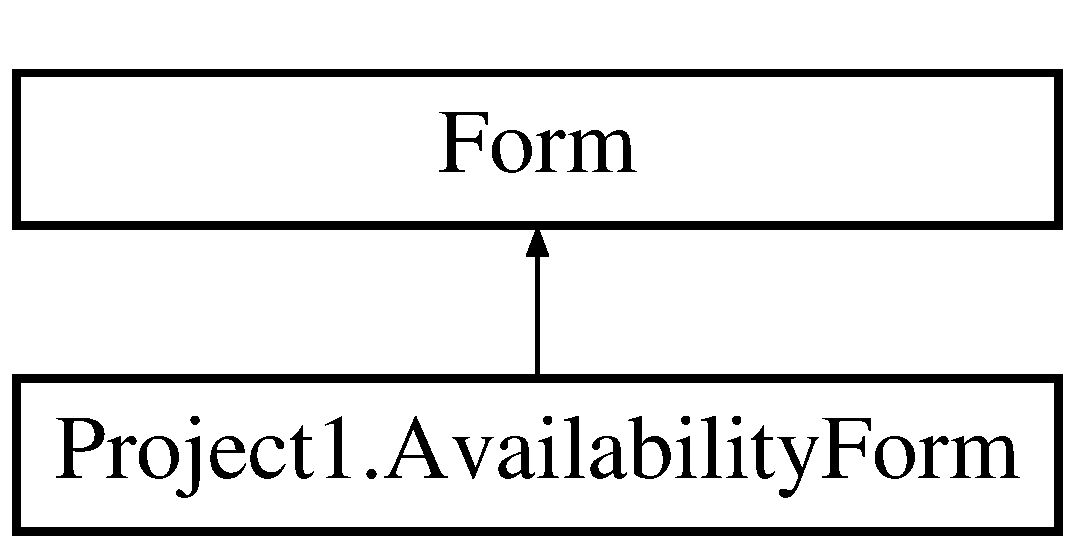
\includegraphics[height=2.000000cm]{classProject1_1_1AvailabilityForm}
\end{center}
\end{figure}
\subsection*{Public Member Functions}
\begin{DoxyCompactItemize}
\item 
\hyperlink{classProject1_1_1AvailabilityForm_af98972a7bdd3aac1c90a011d12e20634}{Availability\+Form} (\hyperlink{classProject1_1_1MainWindow}{Main\+Window} m)
\begin{DoxyCompactList}\small\item\em Initializes a new instance of the \hyperlink{classProject1_1_1AvailabilityForm}{Availability\+Form} class. \end{DoxyCompactList}\end{DoxyCompactItemize}
\subsection*{Protected Member Functions}
\begin{DoxyCompactItemize}
\item 
override void \hyperlink{classProject1_1_1AvailabilityForm_a8f5f4544312a07be4a5c18a0c5f7f57b}{Dispose} (bool disposing)
\begin{DoxyCompactList}\small\item\em Clean up any resources being used. \end{DoxyCompactList}\end{DoxyCompactItemize}
\subsection*{Private Member Functions}
\begin{DoxyCompactItemize}
\item 
void \hyperlink{classProject1_1_1AvailabilityForm_a81c994e26bad20a9a3117f921df3ddd6}{Availability\+Form\+\_\+\+Load\+\_\+1} (object sender, Event\+Args e)
\begin{DoxyCompactList}\small\item\em Handles the 1 event of the Availability\+Form\+\_\+\+Load control. \end{DoxyCompactList}\item 
void \hyperlink{classProject1_1_1AvailabilityForm_ad48d58c06771dc092941ebbeea059895}{check\+Box1\+\_\+\+Checked\+Changed} (object sender, Event\+Args e)
\begin{DoxyCompactList}\small\item\em Handles the Checked\+Changed event of the check\+Box1 control. \end{DoxyCompactList}\item 
void \hyperlink{classProject1_1_1AvailabilityForm_a4e66b612387c8207da934e1667947063}{add\+Button\+\_\+\+Click} (object sender, Event\+Args e)
\begin{DoxyCompactList}\small\item\em Handles the Click event of the add\+Button control. \end{DoxyCompactList}\item 
void \hyperlink{classProject1_1_1AvailabilityForm_a1ad0da6ac770635494b441c775a4f0d5}{events\+Box\+\_\+\+Selected\+Index\+Changed} (object sender, Event\+Args e)
\begin{DoxyCompactList}\small\item\em Handles the Selected\+Index\+Changed event of the events\+Box control. \end{DoxyCompactList}\item 
void \hyperlink{classProject1_1_1AvailabilityForm_aefcd030d389cf6e1882c74d171de373a}{attendee\+Button\+\_\+\+Click} (object sender, Event\+Args e)
\begin{DoxyCompactList}\small\item\em Handles the Click event of the attendee\+Button control. \end{DoxyCompactList}\item 
Date\+Time \mbox{[}$\,$\mbox{]} \hyperlink{classProject1_1_1AvailabilityForm_ae17fdf43349c4e89983592435fc0cc16}{Time\+Slots} ()
\begin{DoxyCompactList}\small\item\em Times the slots. \end{DoxyCompactList}\item 
void \hyperlink{classProject1_1_1AvailabilityForm_a8e5527c2a2732aa00b88e8099f181ac4}{clear\+Button\+\_\+\+Click} (object sender, Event\+Args e)
\begin{DoxyCompactList}\small\item\em Handles the Click event of the clear\+Button control. \end{DoxyCompactList}\item 
void \hyperlink{classProject1_1_1AvailabilityForm_af75b44f7bbfe72fcfbe25b41504eb52d}{Initialize\+Component} ()
\begin{DoxyCompactList}\small\item\em Required method for Designer support -\/ do not modify the contents of this method with the code editor. \end{DoxyCompactList}\end{DoxyCompactItemize}
\subsection*{Private Attributes}
\begin{DoxyCompactItemize}
\item 
\hyperlink{classProject1_1_1MainWindow}{Main\+Window} \hyperlink{classProject1_1_1AvailabilityForm_a419ed9676deb632263bb8c6c74e018e0}{main}
\begin{DoxyCompactList}\small\item\em The main \end{DoxyCompactList}\item 
System.\+Component\+Model.\+I\+Container \hyperlink{classProject1_1_1AvailabilityForm_a929fcebbd2314eb26d638c445aba4d7f}{components} = null
\begin{DoxyCompactList}\small\item\em Required designer variable. \end{DoxyCompactList}\item 
System.\+Windows.\+Forms.\+Button \hyperlink{classProject1_1_1AvailabilityForm_a22eb22776a89cf96b9082108d98b590b}{attendee\+Button}
\item 
System.\+Windows.\+Forms.\+Combo\+Box \hyperlink{classProject1_1_1AvailabilityForm_a57dbb49a194b4b5c1fa4d3efab2eeb1c}{events\+Box}
\item 
System.\+Windows.\+Forms.\+Label \hyperlink{classProject1_1_1AvailabilityForm_aa64d6a18cee83f2e0fcc2190814bc343}{label1}
\item 
System.\+Windows.\+Forms.\+Label \hyperlink{classProject1_1_1AvailabilityForm_ac6fe189a297a1d04f4534257c02a7935}{label2}
\item 
System.\+Windows.\+Forms.\+Text\+Box \hyperlink{classProject1_1_1AvailabilityForm_a039d2e571e7240411359ea4687f45286}{name\+Box}
\item 
System.\+Windows.\+Forms.\+Label \hyperlink{classProject1_1_1AvailabilityForm_a0400b09173c591503c6829ee0eaf6f7e}{label3}
\item 
System.\+Windows.\+Forms.\+Check\+Box \hyperlink{classProject1_1_1AvailabilityForm_ad9cb659cfcfad769b22438a66b0d2536}{check\+Box1}
\item 
System.\+Windows.\+Forms.\+List\+Box \hyperlink{classProject1_1_1AvailabilityForm_ab81f223485ff3facaaf21ed7471d236c}{list\+Box1}
\item 
System.\+Windows.\+Forms.\+Button \hyperlink{classProject1_1_1AvailabilityForm_a636f4b3dee36ddf9496284f2880f3295}{add\+Button}
\item 
System.\+Windows.\+Forms.\+Combo\+Box \hyperlink{classProject1_1_1AvailabilityForm_ade05a84a3b2f475e58385e13f2a35f38}{times\+Box}
\item 
System.\+Windows.\+Forms.\+Button \hyperlink{classProject1_1_1AvailabilityForm_addb714f21b742224d959b2e7ff167583}{clear\+Button}
\end{DoxyCompactItemize}


\subsection{Detailed Description}
Form for adding availability 

\begin{DoxySeeAlso}{See also}
System.\+Windows.\+Forms.\+Form


\end{DoxySeeAlso}


\subsection{Constructor \& Destructor Documentation}
\mbox{\Hypertarget{classProject1_1_1AvailabilityForm_af98972a7bdd3aac1c90a011d12e20634}\label{classProject1_1_1AvailabilityForm_af98972a7bdd3aac1c90a011d12e20634}} 
\index{Project1\+::\+Availability\+Form@{Project1\+::\+Availability\+Form}!Availability\+Form@{Availability\+Form}}
\index{Availability\+Form@{Availability\+Form}!Project1\+::\+Availability\+Form@{Project1\+::\+Availability\+Form}}
\subsubsection{\texorpdfstring{Availability\+Form()}{AvailabilityForm()}}
{\footnotesize\ttfamily Project1.\+Availability\+Form.\+Availability\+Form (\begin{DoxyParamCaption}\item[{\hyperlink{classProject1_1_1MainWindow}{Main\+Window}}]{m }\end{DoxyParamCaption})\hspace{0.3cm}{\ttfamily [inline]}}



Initializes a new instance of the \hyperlink{classProject1_1_1AvailabilityForm}{Availability\+Form} class. 


\begin{DoxyParams}{Parameters}
{\em m} & The m.\\
\hline
\end{DoxyParams}


\subsection{Member Function Documentation}
\mbox{\Hypertarget{classProject1_1_1AvailabilityForm_a4e66b612387c8207da934e1667947063}\label{classProject1_1_1AvailabilityForm_a4e66b612387c8207da934e1667947063}} 
\index{Project1\+::\+Availability\+Form@{Project1\+::\+Availability\+Form}!add\+Button\+\_\+\+Click@{add\+Button\+\_\+\+Click}}
\index{add\+Button\+\_\+\+Click@{add\+Button\+\_\+\+Click}!Project1\+::\+Availability\+Form@{Project1\+::\+Availability\+Form}}
\subsubsection{\texorpdfstring{add\+Button\+\_\+\+Click()}{addButton\_Click()}}
{\footnotesize\ttfamily void Project1.\+Availability\+Form.\+add\+Button\+\_\+\+Click (\begin{DoxyParamCaption}\item[{object}]{sender,  }\item[{Event\+Args}]{e }\end{DoxyParamCaption})\hspace{0.3cm}{\ttfamily [inline]}, {\ttfamily [private]}}



Handles the Click event of the add\+Button control. 


\begin{DoxyParams}{Parameters}
{\em sender} & The source of the event.\\
\hline
{\em e} & The Event\+Args instance containing the event data.\\
\hline
\end{DoxyParams}
\mbox{\Hypertarget{classProject1_1_1AvailabilityForm_aefcd030d389cf6e1882c74d171de373a}\label{classProject1_1_1AvailabilityForm_aefcd030d389cf6e1882c74d171de373a}} 
\index{Project1\+::\+Availability\+Form@{Project1\+::\+Availability\+Form}!attendee\+Button\+\_\+\+Click@{attendee\+Button\+\_\+\+Click}}
\index{attendee\+Button\+\_\+\+Click@{attendee\+Button\+\_\+\+Click}!Project1\+::\+Availability\+Form@{Project1\+::\+Availability\+Form}}
\subsubsection{\texorpdfstring{attendee\+Button\+\_\+\+Click()}{attendeeButton\_Click()}}
{\footnotesize\ttfamily void Project1.\+Availability\+Form.\+attendee\+Button\+\_\+\+Click (\begin{DoxyParamCaption}\item[{object}]{sender,  }\item[{Event\+Args}]{e }\end{DoxyParamCaption})\hspace{0.3cm}{\ttfamily [inline]}, {\ttfamily [private]}}



Handles the Click event of the attendee\+Button control. 


\begin{DoxyParams}{Parameters}
{\em sender} & The source of the event.\\
\hline
{\em e} & The Event\+Args instance containing the event data.\\
\hline
\end{DoxyParams}
\mbox{\Hypertarget{classProject1_1_1AvailabilityForm_a81c994e26bad20a9a3117f921df3ddd6}\label{classProject1_1_1AvailabilityForm_a81c994e26bad20a9a3117f921df3ddd6}} 
\index{Project1\+::\+Availability\+Form@{Project1\+::\+Availability\+Form}!Availability\+Form\+\_\+\+Load\+\_\+1@{Availability\+Form\+\_\+\+Load\+\_\+1}}
\index{Availability\+Form\+\_\+\+Load\+\_\+1@{Availability\+Form\+\_\+\+Load\+\_\+1}!Project1\+::\+Availability\+Form@{Project1\+::\+Availability\+Form}}
\subsubsection{\texorpdfstring{Availability\+Form\+\_\+\+Load\+\_\+1()}{AvailabilityForm\_Load\_1()}}
{\footnotesize\ttfamily void Project1.\+Availability\+Form.\+Availability\+Form\+\_\+\+Load\+\_\+1 (\begin{DoxyParamCaption}\item[{object}]{sender,  }\item[{Event\+Args}]{e }\end{DoxyParamCaption})\hspace{0.3cm}{\ttfamily [inline]}, {\ttfamily [private]}}



Handles the 1 event of the Availability\+Form\+\_\+\+Load control. 


\begin{DoxyParams}{Parameters}
{\em sender} & The source of the event.\\
\hline
{\em e} & The Event\+Args instance containing the event data.\\
\hline
\end{DoxyParams}
\mbox{\Hypertarget{classProject1_1_1AvailabilityForm_ad48d58c06771dc092941ebbeea059895}\label{classProject1_1_1AvailabilityForm_ad48d58c06771dc092941ebbeea059895}} 
\index{Project1\+::\+Availability\+Form@{Project1\+::\+Availability\+Form}!check\+Box1\+\_\+\+Checked\+Changed@{check\+Box1\+\_\+\+Checked\+Changed}}
\index{check\+Box1\+\_\+\+Checked\+Changed@{check\+Box1\+\_\+\+Checked\+Changed}!Project1\+::\+Availability\+Form@{Project1\+::\+Availability\+Form}}
\subsubsection{\texorpdfstring{check\+Box1\+\_\+\+Checked\+Changed()}{checkBox1\_CheckedChanged()}}
{\footnotesize\ttfamily void Project1.\+Availability\+Form.\+check\+Box1\+\_\+\+Checked\+Changed (\begin{DoxyParamCaption}\item[{object}]{sender,  }\item[{Event\+Args}]{e }\end{DoxyParamCaption})\hspace{0.3cm}{\ttfamily [inline]}, {\ttfamily [private]}}



Handles the Checked\+Changed event of the check\+Box1 control. 


\begin{DoxyParams}{Parameters}
{\em sender} & The source of the event.\\
\hline
{\em e} & The Event\+Args instance containing the event data.\\
\hline
\end{DoxyParams}
\mbox{\Hypertarget{classProject1_1_1AvailabilityForm_a8e5527c2a2732aa00b88e8099f181ac4}\label{classProject1_1_1AvailabilityForm_a8e5527c2a2732aa00b88e8099f181ac4}} 
\index{Project1\+::\+Availability\+Form@{Project1\+::\+Availability\+Form}!clear\+Button\+\_\+\+Click@{clear\+Button\+\_\+\+Click}}
\index{clear\+Button\+\_\+\+Click@{clear\+Button\+\_\+\+Click}!Project1\+::\+Availability\+Form@{Project1\+::\+Availability\+Form}}
\subsubsection{\texorpdfstring{clear\+Button\+\_\+\+Click()}{clearButton\_Click()}}
{\footnotesize\ttfamily void Project1.\+Availability\+Form.\+clear\+Button\+\_\+\+Click (\begin{DoxyParamCaption}\item[{object}]{sender,  }\item[{Event\+Args}]{e }\end{DoxyParamCaption})\hspace{0.3cm}{\ttfamily [inline]}, {\ttfamily [private]}}



Handles the Click event of the clear\+Button control. 


\begin{DoxyParams}{Parameters}
{\em sender} & The source of the event.\\
\hline
{\em e} & The Event\+Args instance containing the event data.\\
\hline
\end{DoxyParams}
\mbox{\Hypertarget{classProject1_1_1AvailabilityForm_a8f5f4544312a07be4a5c18a0c5f7f57b}\label{classProject1_1_1AvailabilityForm_a8f5f4544312a07be4a5c18a0c5f7f57b}} 
\index{Project1\+::\+Availability\+Form@{Project1\+::\+Availability\+Form}!Dispose@{Dispose}}
\index{Dispose@{Dispose}!Project1\+::\+Availability\+Form@{Project1\+::\+Availability\+Form}}
\subsubsection{\texorpdfstring{Dispose()}{Dispose()}}
{\footnotesize\ttfamily override void Project1.\+Availability\+Form.\+Dispose (\begin{DoxyParamCaption}\item[{bool}]{disposing }\end{DoxyParamCaption})\hspace{0.3cm}{\ttfamily [inline]}, {\ttfamily [protected]}}



Clean up any resources being used. 


\begin{DoxyParams}{Parameters}
{\em disposing} & true if managed resources should be disposed; otherwise, false.\\
\hline
\end{DoxyParams}
\mbox{\Hypertarget{classProject1_1_1AvailabilityForm_a1ad0da6ac770635494b441c775a4f0d5}\label{classProject1_1_1AvailabilityForm_a1ad0da6ac770635494b441c775a4f0d5}} 
\index{Project1\+::\+Availability\+Form@{Project1\+::\+Availability\+Form}!events\+Box\+\_\+\+Selected\+Index\+Changed@{events\+Box\+\_\+\+Selected\+Index\+Changed}}
\index{events\+Box\+\_\+\+Selected\+Index\+Changed@{events\+Box\+\_\+\+Selected\+Index\+Changed}!Project1\+::\+Availability\+Form@{Project1\+::\+Availability\+Form}}
\subsubsection{\texorpdfstring{events\+Box\+\_\+\+Selected\+Index\+Changed()}{eventsBox\_SelectedIndexChanged()}}
{\footnotesize\ttfamily void Project1.\+Availability\+Form.\+events\+Box\+\_\+\+Selected\+Index\+Changed (\begin{DoxyParamCaption}\item[{object}]{sender,  }\item[{Event\+Args}]{e }\end{DoxyParamCaption})\hspace{0.3cm}{\ttfamily [inline]}, {\ttfamily [private]}}



Handles the Selected\+Index\+Changed event of the events\+Box control. 


\begin{DoxyParams}{Parameters}
{\em sender} & The source of the event.\\
\hline
{\em e} & The Event\+Args instance containing the event data.\\
\hline
\end{DoxyParams}
\mbox{\Hypertarget{classProject1_1_1AvailabilityForm_af75b44f7bbfe72fcfbe25b41504eb52d}\label{classProject1_1_1AvailabilityForm_af75b44f7bbfe72fcfbe25b41504eb52d}} 
\index{Project1\+::\+Availability\+Form@{Project1\+::\+Availability\+Form}!Initialize\+Component@{Initialize\+Component}}
\index{Initialize\+Component@{Initialize\+Component}!Project1\+::\+Availability\+Form@{Project1\+::\+Availability\+Form}}
\subsubsection{\texorpdfstring{Initialize\+Component()}{InitializeComponent()}}
{\footnotesize\ttfamily void Project1.\+Availability\+Form.\+Initialize\+Component (\begin{DoxyParamCaption}{ }\end{DoxyParamCaption})\hspace{0.3cm}{\ttfamily [inline]}, {\ttfamily [private]}}



Required method for Designer support -\/ do not modify the contents of this method with the code editor. 

\mbox{\Hypertarget{classProject1_1_1AvailabilityForm_ae17fdf43349c4e89983592435fc0cc16}\label{classProject1_1_1AvailabilityForm_ae17fdf43349c4e89983592435fc0cc16}} 
\index{Project1\+::\+Availability\+Form@{Project1\+::\+Availability\+Form}!Time\+Slots@{Time\+Slots}}
\index{Time\+Slots@{Time\+Slots}!Project1\+::\+Availability\+Form@{Project1\+::\+Availability\+Form}}
\subsubsection{\texorpdfstring{Time\+Slots()}{TimeSlots()}}
{\footnotesize\ttfamily Date\+Time \mbox{[}$\,$\mbox{]} Project1.\+Availability\+Form.\+Time\+Slots (\begin{DoxyParamCaption}{ }\end{DoxyParamCaption})\hspace{0.3cm}{\ttfamily [inline]}, {\ttfamily [private]}}



Times the slots. 

\begin{DoxyReturn}{Returns}

\end{DoxyReturn}


\subsection{Member Data Documentation}
\mbox{\Hypertarget{classProject1_1_1AvailabilityForm_a636f4b3dee36ddf9496284f2880f3295}\label{classProject1_1_1AvailabilityForm_a636f4b3dee36ddf9496284f2880f3295}} 
\index{Project1\+::\+Availability\+Form@{Project1\+::\+Availability\+Form}!add\+Button@{add\+Button}}
\index{add\+Button@{add\+Button}!Project1\+::\+Availability\+Form@{Project1\+::\+Availability\+Form}}
\subsubsection{\texorpdfstring{add\+Button}{addButton}}
{\footnotesize\ttfamily System.\+Windows.\+Forms.\+Button Project1.\+Availability\+Form.\+add\+Button\hspace{0.3cm}{\ttfamily [private]}}

\mbox{\Hypertarget{classProject1_1_1AvailabilityForm_a22eb22776a89cf96b9082108d98b590b}\label{classProject1_1_1AvailabilityForm_a22eb22776a89cf96b9082108d98b590b}} 
\index{Project1\+::\+Availability\+Form@{Project1\+::\+Availability\+Form}!attendee\+Button@{attendee\+Button}}
\index{attendee\+Button@{attendee\+Button}!Project1\+::\+Availability\+Form@{Project1\+::\+Availability\+Form}}
\subsubsection{\texorpdfstring{attendee\+Button}{attendeeButton}}
{\footnotesize\ttfamily System.\+Windows.\+Forms.\+Button Project1.\+Availability\+Form.\+attendee\+Button\hspace{0.3cm}{\ttfamily [private]}}

\mbox{\Hypertarget{classProject1_1_1AvailabilityForm_ad9cb659cfcfad769b22438a66b0d2536}\label{classProject1_1_1AvailabilityForm_ad9cb659cfcfad769b22438a66b0d2536}} 
\index{Project1\+::\+Availability\+Form@{Project1\+::\+Availability\+Form}!check\+Box1@{check\+Box1}}
\index{check\+Box1@{check\+Box1}!Project1\+::\+Availability\+Form@{Project1\+::\+Availability\+Form}}
\subsubsection{\texorpdfstring{check\+Box1}{checkBox1}}
{\footnotesize\ttfamily System.\+Windows.\+Forms.\+Check\+Box Project1.\+Availability\+Form.\+check\+Box1\hspace{0.3cm}{\ttfamily [private]}}

\mbox{\Hypertarget{classProject1_1_1AvailabilityForm_addb714f21b742224d959b2e7ff167583}\label{classProject1_1_1AvailabilityForm_addb714f21b742224d959b2e7ff167583}} 
\index{Project1\+::\+Availability\+Form@{Project1\+::\+Availability\+Form}!clear\+Button@{clear\+Button}}
\index{clear\+Button@{clear\+Button}!Project1\+::\+Availability\+Form@{Project1\+::\+Availability\+Form}}
\subsubsection{\texorpdfstring{clear\+Button}{clearButton}}
{\footnotesize\ttfamily System.\+Windows.\+Forms.\+Button Project1.\+Availability\+Form.\+clear\+Button\hspace{0.3cm}{\ttfamily [private]}}

\mbox{\Hypertarget{classProject1_1_1AvailabilityForm_a929fcebbd2314eb26d638c445aba4d7f}\label{classProject1_1_1AvailabilityForm_a929fcebbd2314eb26d638c445aba4d7f}} 
\index{Project1\+::\+Availability\+Form@{Project1\+::\+Availability\+Form}!components@{components}}
\index{components@{components}!Project1\+::\+Availability\+Form@{Project1\+::\+Availability\+Form}}
\subsubsection{\texorpdfstring{components}{components}}
{\footnotesize\ttfamily System.\+Component\+Model.\+I\+Container Project1.\+Availability\+Form.\+components = null\hspace{0.3cm}{\ttfamily [private]}}



Required designer variable. 

\mbox{\Hypertarget{classProject1_1_1AvailabilityForm_a57dbb49a194b4b5c1fa4d3efab2eeb1c}\label{classProject1_1_1AvailabilityForm_a57dbb49a194b4b5c1fa4d3efab2eeb1c}} 
\index{Project1\+::\+Availability\+Form@{Project1\+::\+Availability\+Form}!events\+Box@{events\+Box}}
\index{events\+Box@{events\+Box}!Project1\+::\+Availability\+Form@{Project1\+::\+Availability\+Form}}
\subsubsection{\texorpdfstring{events\+Box}{eventsBox}}
{\footnotesize\ttfamily System.\+Windows.\+Forms.\+Combo\+Box Project1.\+Availability\+Form.\+events\+Box\hspace{0.3cm}{\ttfamily [private]}}

\mbox{\Hypertarget{classProject1_1_1AvailabilityForm_aa64d6a18cee83f2e0fcc2190814bc343}\label{classProject1_1_1AvailabilityForm_aa64d6a18cee83f2e0fcc2190814bc343}} 
\index{Project1\+::\+Availability\+Form@{Project1\+::\+Availability\+Form}!label1@{label1}}
\index{label1@{label1}!Project1\+::\+Availability\+Form@{Project1\+::\+Availability\+Form}}
\subsubsection{\texorpdfstring{label1}{label1}}
{\footnotesize\ttfamily System.\+Windows.\+Forms.\+Label Project1.\+Availability\+Form.\+label1\hspace{0.3cm}{\ttfamily [private]}}

\mbox{\Hypertarget{classProject1_1_1AvailabilityForm_ac6fe189a297a1d04f4534257c02a7935}\label{classProject1_1_1AvailabilityForm_ac6fe189a297a1d04f4534257c02a7935}} 
\index{Project1\+::\+Availability\+Form@{Project1\+::\+Availability\+Form}!label2@{label2}}
\index{label2@{label2}!Project1\+::\+Availability\+Form@{Project1\+::\+Availability\+Form}}
\subsubsection{\texorpdfstring{label2}{label2}}
{\footnotesize\ttfamily System.\+Windows.\+Forms.\+Label Project1.\+Availability\+Form.\+label2\hspace{0.3cm}{\ttfamily [private]}}

\mbox{\Hypertarget{classProject1_1_1AvailabilityForm_a0400b09173c591503c6829ee0eaf6f7e}\label{classProject1_1_1AvailabilityForm_a0400b09173c591503c6829ee0eaf6f7e}} 
\index{Project1\+::\+Availability\+Form@{Project1\+::\+Availability\+Form}!label3@{label3}}
\index{label3@{label3}!Project1\+::\+Availability\+Form@{Project1\+::\+Availability\+Form}}
\subsubsection{\texorpdfstring{label3}{label3}}
{\footnotesize\ttfamily System.\+Windows.\+Forms.\+Label Project1.\+Availability\+Form.\+label3\hspace{0.3cm}{\ttfamily [private]}}

\mbox{\Hypertarget{classProject1_1_1AvailabilityForm_ab81f223485ff3facaaf21ed7471d236c}\label{classProject1_1_1AvailabilityForm_ab81f223485ff3facaaf21ed7471d236c}} 
\index{Project1\+::\+Availability\+Form@{Project1\+::\+Availability\+Form}!list\+Box1@{list\+Box1}}
\index{list\+Box1@{list\+Box1}!Project1\+::\+Availability\+Form@{Project1\+::\+Availability\+Form}}
\subsubsection{\texorpdfstring{list\+Box1}{listBox1}}
{\footnotesize\ttfamily System.\+Windows.\+Forms.\+List\+Box Project1.\+Availability\+Form.\+list\+Box1\hspace{0.3cm}{\ttfamily [private]}}

\mbox{\Hypertarget{classProject1_1_1AvailabilityForm_a419ed9676deb632263bb8c6c74e018e0}\label{classProject1_1_1AvailabilityForm_a419ed9676deb632263bb8c6c74e018e0}} 
\index{Project1\+::\+Availability\+Form@{Project1\+::\+Availability\+Form}!main@{main}}
\index{main@{main}!Project1\+::\+Availability\+Form@{Project1\+::\+Availability\+Form}}
\subsubsection{\texorpdfstring{main}{main}}
{\footnotesize\ttfamily \hyperlink{classProject1_1_1MainWindow}{Main\+Window} Project1.\+Availability\+Form.\+main\hspace{0.3cm}{\ttfamily [private]}}



The main 

\mbox{\Hypertarget{classProject1_1_1AvailabilityForm_a039d2e571e7240411359ea4687f45286}\label{classProject1_1_1AvailabilityForm_a039d2e571e7240411359ea4687f45286}} 
\index{Project1\+::\+Availability\+Form@{Project1\+::\+Availability\+Form}!name\+Box@{name\+Box}}
\index{name\+Box@{name\+Box}!Project1\+::\+Availability\+Form@{Project1\+::\+Availability\+Form}}
\subsubsection{\texorpdfstring{name\+Box}{nameBox}}
{\footnotesize\ttfamily System.\+Windows.\+Forms.\+Text\+Box Project1.\+Availability\+Form.\+name\+Box\hspace{0.3cm}{\ttfamily [private]}}

\mbox{\Hypertarget{classProject1_1_1AvailabilityForm_ade05a84a3b2f475e58385e13f2a35f38}\label{classProject1_1_1AvailabilityForm_ade05a84a3b2f475e58385e13f2a35f38}} 
\index{Project1\+::\+Availability\+Form@{Project1\+::\+Availability\+Form}!times\+Box@{times\+Box}}
\index{times\+Box@{times\+Box}!Project1\+::\+Availability\+Form@{Project1\+::\+Availability\+Form}}
\subsubsection{\texorpdfstring{times\+Box}{timesBox}}
{\footnotesize\ttfamily System.\+Windows.\+Forms.\+Combo\+Box Project1.\+Availability\+Form.\+times\+Box\hspace{0.3cm}{\ttfamily [private]}}



The documentation for this class was generated from the following files\+:\begin{DoxyCompactItemize}
\item 
Project1/\hyperlink{AvailabilityForm_8cs}{Availability\+Form.\+cs}\item 
Project1/\hyperlink{AvailabilityForm_8Designer_8cs}{Availability\+Form.\+Designer.\+cs}\end{DoxyCompactItemize}

\hypertarget{classProject1_1_1Event}{}\section{Project1.\+Event Class Reference}
\label{classProject1_1_1Event}\index{Project1.\+Event@{Project1.\+Event}}


\hyperlink{classProject1_1_1Event}{Event} class  


\subsection*{Public Member Functions}
\begin{DoxyCompactItemize}
\item 
\hyperlink{classProject1_1_1Event_a55c477aa9e921902fd85ff505c93b661}{Event} (string Host, string Name, Date\+Time Date, Date\+Time\mbox{[}$\,$\mbox{]} Times)
\begin{DoxyCompactList}\small\item\em Initializes a new instance of the \hyperlink{classProject1_1_1Event}{Event} class. \end{DoxyCompactList}\item 
override string \hyperlink{classProject1_1_1Event_a0e234eb98d62ce49bd5ed4c658e307ff}{To\+String} ()
\begin{DoxyCompactList}\small\item\em Returns a System.\+String that represents this instance. \end{DoxyCompactList}\end{DoxyCompactItemize}
\subsection*{Public Attributes}
\begin{DoxyCompactItemize}
\item 
List$<$ \hyperlink{classProject1_1_1Attendee}{Attendee} $>$ \hyperlink{classProject1_1_1Event_ab84e6fa3b0d021689d80c02e4d23731b}{attendees} = new List$<$\hyperlink{classProject1_1_1Attendee}{Attendee}$>$()
\begin{DoxyCompactList}\small\item\em The attendees \end{DoxyCompactList}\end{DoxyCompactItemize}
\subsection*{Properties}
\begin{DoxyCompactItemize}
\item 
String \hyperlink{classProject1_1_1Event_a04f15bb124d4410eece35779864589bf}{name}\hspace{0.3cm}{\ttfamily  \mbox{[}get, private set\mbox{]}}
\begin{DoxyCompactList}\small\item\em Gets the name. \end{DoxyCompactList}\item 
String \hyperlink{classProject1_1_1Event_a50ac8e67c15316ea93bcbca4b7951fee}{host}\hspace{0.3cm}{\ttfamily  \mbox{[}get, private set\mbox{]}}
\begin{DoxyCompactList}\small\item\em Gets the host. \end{DoxyCompactList}\item 
Date\+Time \hyperlink{classProject1_1_1Event_a4a7ca6b514ebc64a364c4aac4c7a3b5f}{date}\hspace{0.3cm}{\ttfamily  \mbox{[}get, private set\mbox{]}}
\begin{DoxyCompactList}\small\item\em Gets the date. \end{DoxyCompactList}\item 
Date\+Time \mbox{[}$\,$\mbox{]} \hyperlink{classProject1_1_1Event_acc6d286c687a5ac9256a146d99de1cb6}{times}\hspace{0.3cm}{\ttfamily  \mbox{[}get, private set\mbox{]}}
\begin{DoxyCompactList}\small\item\em Gets the times. \end{DoxyCompactList}\end{DoxyCompactItemize}


\subsection{Detailed Description}
\hyperlink{classProject1_1_1Event}{Event} class 



\subsection{Constructor \& Destructor Documentation}
\mbox{\Hypertarget{classProject1_1_1Event_a55c477aa9e921902fd85ff505c93b661}\label{classProject1_1_1Event_a55c477aa9e921902fd85ff505c93b661}} 
\index{Project1\+::\+Event@{Project1\+::\+Event}!Event@{Event}}
\index{Event@{Event}!Project1\+::\+Event@{Project1\+::\+Event}}
\subsubsection{\texorpdfstring{Event()}{Event()}}
{\footnotesize\ttfamily Project1.\+Event.\+Event (\begin{DoxyParamCaption}\item[{string}]{Host,  }\item[{string}]{Name,  }\item[{Date\+Time}]{Date,  }\item[{Date\+Time \mbox{[}$\,$\mbox{]}}]{Times }\end{DoxyParamCaption})\hspace{0.3cm}{\ttfamily [inline]}}



Initializes a new instance of the \hyperlink{classProject1_1_1Event}{Event} class. 


\begin{DoxyParams}{Parameters}
{\em Host} & The host.\\
\hline
{\em Name} & The name.\\
\hline
{\em Date} & The date.\\
\hline
{\em Times} & The times.\\
\hline
\end{DoxyParams}


\subsection{Member Function Documentation}
\mbox{\Hypertarget{classProject1_1_1Event_a0e234eb98d62ce49bd5ed4c658e307ff}\label{classProject1_1_1Event_a0e234eb98d62ce49bd5ed4c658e307ff}} 
\index{Project1\+::\+Event@{Project1\+::\+Event}!To\+String@{To\+String}}
\index{To\+String@{To\+String}!Project1\+::\+Event@{Project1\+::\+Event}}
\subsubsection{\texorpdfstring{To\+String()}{ToString()}}
{\footnotesize\ttfamily override string Project1.\+Event.\+To\+String (\begin{DoxyParamCaption}{ }\end{DoxyParamCaption})\hspace{0.3cm}{\ttfamily [inline]}}



Returns a System.\+String that represents this instance. 

\begin{DoxyReturn}{Returns}
A System.\+String that represents this instance. 
\end{DoxyReturn}


\subsection{Member Data Documentation}
\mbox{\Hypertarget{classProject1_1_1Event_ab84e6fa3b0d021689d80c02e4d23731b}\label{classProject1_1_1Event_ab84e6fa3b0d021689d80c02e4d23731b}} 
\index{Project1\+::\+Event@{Project1\+::\+Event}!attendees@{attendees}}
\index{attendees@{attendees}!Project1\+::\+Event@{Project1\+::\+Event}}
\subsubsection{\texorpdfstring{attendees}{attendees}}
{\footnotesize\ttfamily List$<$\hyperlink{classProject1_1_1Attendee}{Attendee}$>$ Project1.\+Event.\+attendees = new List$<$\hyperlink{classProject1_1_1Attendee}{Attendee}$>$()}



The attendees 



\subsection{Property Documentation}
\mbox{\Hypertarget{classProject1_1_1Event_a4a7ca6b514ebc64a364c4aac4c7a3b5f}\label{classProject1_1_1Event_a4a7ca6b514ebc64a364c4aac4c7a3b5f}} 
\index{Project1\+::\+Event@{Project1\+::\+Event}!date@{date}}
\index{date@{date}!Project1\+::\+Event@{Project1\+::\+Event}}
\subsubsection{\texorpdfstring{date}{date}}
{\footnotesize\ttfamily Date\+Time Project1.\+Event.\+date\hspace{0.3cm}{\ttfamily [get]}, {\ttfamily [private set]}}



Gets the date. 

The date. \mbox{\Hypertarget{classProject1_1_1Event_a50ac8e67c15316ea93bcbca4b7951fee}\label{classProject1_1_1Event_a50ac8e67c15316ea93bcbca4b7951fee}} 
\index{Project1\+::\+Event@{Project1\+::\+Event}!host@{host}}
\index{host@{host}!Project1\+::\+Event@{Project1\+::\+Event}}
\subsubsection{\texorpdfstring{host}{host}}
{\footnotesize\ttfamily String Project1.\+Event.\+host\hspace{0.3cm}{\ttfamily [get]}, {\ttfamily [private set]}}



Gets the host. 

The host. \mbox{\Hypertarget{classProject1_1_1Event_a04f15bb124d4410eece35779864589bf}\label{classProject1_1_1Event_a04f15bb124d4410eece35779864589bf}} 
\index{Project1\+::\+Event@{Project1\+::\+Event}!name@{name}}
\index{name@{name}!Project1\+::\+Event@{Project1\+::\+Event}}
\subsubsection{\texorpdfstring{name}{name}}
{\footnotesize\ttfamily String Project1.\+Event.\+name\hspace{0.3cm}{\ttfamily [get]}, {\ttfamily [private set]}}



Gets the name. 

The name. \mbox{\Hypertarget{classProject1_1_1Event_acc6d286c687a5ac9256a146d99de1cb6}\label{classProject1_1_1Event_acc6d286c687a5ac9256a146d99de1cb6}} 
\index{Project1\+::\+Event@{Project1\+::\+Event}!times@{times}}
\index{times@{times}!Project1\+::\+Event@{Project1\+::\+Event}}
\subsubsection{\texorpdfstring{times}{times}}
{\footnotesize\ttfamily Date\+Time \mbox{[}$\,$\mbox{]} Project1.\+Event.\+times\hspace{0.3cm}{\ttfamily [get]}, {\ttfamily [private set]}}



Gets the times. 

The times. 

The documentation for this class was generated from the following file\+:\begin{DoxyCompactItemize}
\item 
Project1/\hyperlink{Event_8cs}{Event.\+cs}\end{DoxyCompactItemize}

\hypertarget{classProject1_1_1EventInfo}{}\section{Project1.\+Event\+Info Class Reference}
\label{classProject1_1_1EventInfo}\index{Project1.\+Event\+Info@{Project1.\+Event\+Info}}


The event creation form  


Inheritance diagram for Project1.\+Event\+Info\+:\begin{figure}[H]
\begin{center}
\leavevmode
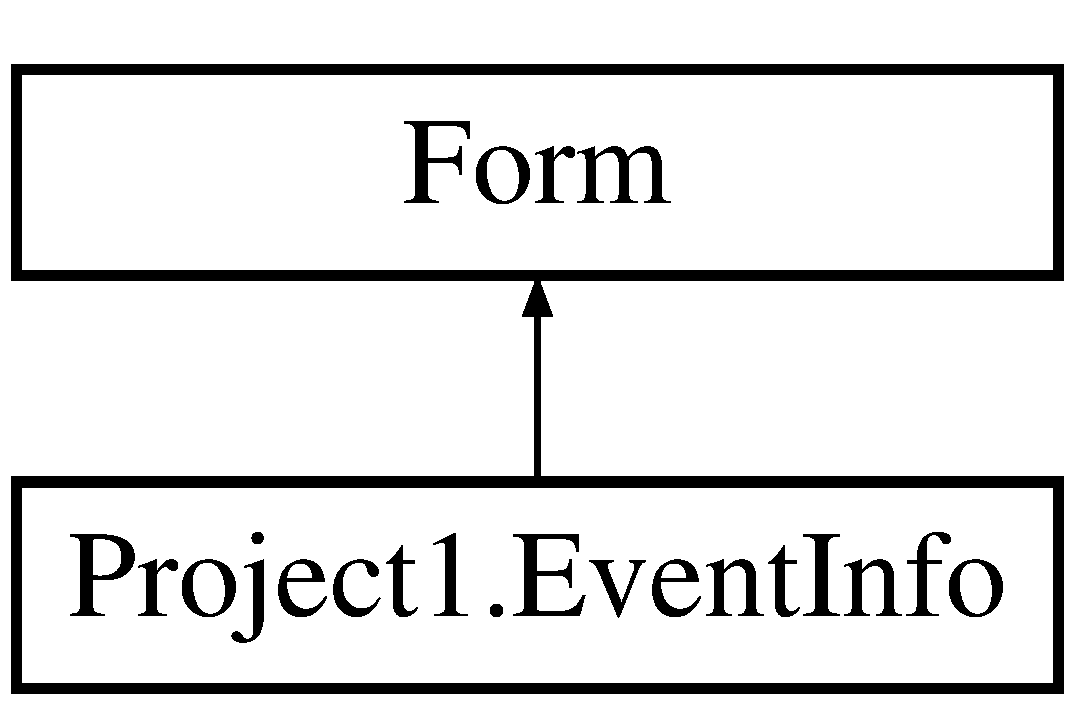
\includegraphics[height=2.000000cm]{classProject1_1_1EventInfo}
\end{center}
\end{figure}
\subsection*{Public Member Functions}
\begin{DoxyCompactItemize}
\item 
\hyperlink{classProject1_1_1EventInfo_a9bf24095fee3d3b879e61fa990e8209c}{Event\+Info} (\hyperlink{classProject1_1_1MainWindow}{Main\+Window} m)
\begin{DoxyCompactList}\small\item\em Passes the \hyperlink{classProject1_1_1MainWindow}{Main\+Window} into this window to allow interaction between the two. \end{DoxyCompactList}\end{DoxyCompactItemize}
\subsection*{Protected Member Functions}
\begin{DoxyCompactItemize}
\item 
override void \hyperlink{classProject1_1_1EventInfo_aa54f1ee810e1b9ea20b3bb9ed76be80b}{Dispose} (bool disposing)
\begin{DoxyCompactList}\small\item\em Clean up any resources being used. \end{DoxyCompactList}\end{DoxyCompactItemize}
\subsection*{Package Attributes}
\begin{DoxyCompactItemize}
\item 
\hyperlink{classProject1_1_1MainWindow}{Main\+Window} \hyperlink{classProject1_1_1EventInfo_ab2930e440128bf910d922e7615676d0d}{main} = null
\begin{DoxyCompactList}\small\item\em The main \end{DoxyCompactList}\end{DoxyCompactItemize}
\subsection*{Private Member Functions}
\begin{DoxyCompactItemize}
\item 
void \hyperlink{classProject1_1_1EventInfo_a7f1582debc3b36848116513dbefb690c}{add\+Button\+\_\+\+Click} (object sender, Event\+Args e)
\begin{DoxyCompactList}\small\item\em Adds a selected time from the time\+Box to the list\+Box. The Item is inserted in ascending order. \end{DoxyCompactList}\item 
void \hyperlink{classProject1_1_1EventInfo_aaa2e7fde2f469c6769b8099941bd66d0}{remove\+Button\+\_\+\+Click} (object sender, Event\+Args e)
\begin{DoxyCompactList}\small\item\em Deletes all time slots from the listbox \end{DoxyCompactList}\item 
void \hyperlink{classProject1_1_1EventInfo_a3b0662eb1959327307b4e4992123378f}{add\+Event\+Button\+\_\+\+Click} (object sender, Event\+Args e)
\begin{DoxyCompactList}\small\item\em Saves event information to a file and checks for correctness. \end{DoxyCompactList}\item 
Date\+Time \mbox{[}$\,$\mbox{]} \hyperlink{classProject1_1_1EventInfo_a12da689af1a5f87c244d014247cf4f73}{Time\+Slots} ()
\begin{DoxyCompactList}\small\item\em Times the slots. \end{DoxyCompactList}\item 
void \hyperlink{classProject1_1_1EventInfo_a3bf5e88c899ab15fbe76bdccc1a72e9d}{Event\+Info\+\_\+\+Load} (object sender, Event\+Args e)
\begin{DoxyCompactList}\small\item\em Adds time slots into combobox for selection in 12 hr format and prevents user from picking an earlier date than today. \end{DoxyCompactList}\item 
void \hyperlink{classProject1_1_1EventInfo_a64e3ce2cb6745b461022d2a968cad153}{check\+Box1\+\_\+\+Checked\+Changed} (object sender, Event\+Args e)
\begin{DoxyCompactList}\small\item\em Changes time format between 24 hr and 12 hr format for combobox and listbox. \end{DoxyCompactList}\item 
void \hyperlink{classProject1_1_1EventInfo_ad8918624e8ae88b80277a9c1b913b1c3}{Initialize\+Component} ()
\begin{DoxyCompactList}\small\item\em Required method for Designer support -\/ do not modify the contents of this method with the code editor. \end{DoxyCompactList}\end{DoxyCompactItemize}
\subsection*{Private Attributes}
\begin{DoxyCompactItemize}
\item 
System.\+Component\+Model.\+I\+Container \hyperlink{classProject1_1_1EventInfo_a70368824a7f92cc152cc1371ebd6e5f1}{components} = null
\begin{DoxyCompactList}\small\item\em Required designer variable. \end{DoxyCompactList}\item 
System.\+Windows.\+Forms.\+Text\+Box \hyperlink{classProject1_1_1EventInfo_ade60ccc9dc0e3789c0323820d368f667}{event\+Name\+Box}
\item 
System.\+Windows.\+Forms.\+Label \hyperlink{classProject1_1_1EventInfo_ab0c0388a63ceddd8ecde61ce4e00ffe8}{label1}
\item 
System.\+Windows.\+Forms.\+Date\+Time\+Picker \hyperlink{classProject1_1_1EventInfo_ad9fd1f5363989b649ffe1681afda852c}{date\+Time\+Picker1}
\item 
System.\+Windows.\+Forms.\+Label \hyperlink{classProject1_1_1EventInfo_a27ead48983981a1f8e4d936ad0a113eb}{label2}
\item 
System.\+Windows.\+Forms.\+Label \hyperlink{classProject1_1_1EventInfo_a5489960f8593264df7d3a32fc362c95e}{label3}
\item 
System.\+Windows.\+Forms.\+List\+Box \hyperlink{classProject1_1_1EventInfo_a229ac9e88dea0086ae9055095dc98da4}{list\+Box1}
\item 
System.\+Windows.\+Forms.\+Button \hyperlink{classProject1_1_1EventInfo_a1b28ec9d90e8ff63e7589515f7b6f64a}{add\+Button}
\item 
System.\+Windows.\+Forms.\+Button \hyperlink{classProject1_1_1EventInfo_ae3ecbf994b93d37b2d6e42fcb0631ef0}{remove\+Button}
\item 
System.\+Windows.\+Forms.\+Check\+Box \hyperlink{classProject1_1_1EventInfo_ace75bf4615d0f8add3e53b6791fb671c}{check\+Box1}
\item 
System.\+Windows.\+Forms.\+Combo\+Box \hyperlink{classProject1_1_1EventInfo_ad368077ede71cc2fb15a34a5a95ac978}{times\+Box}
\item 
System.\+Windows.\+Forms.\+Button \hyperlink{classProject1_1_1EventInfo_a3a841021c735952afd4c491508540c62}{add\+Event\+Button}
\item 
System.\+Windows.\+Forms.\+Label \hyperlink{classProject1_1_1EventInfo_ac29d91498e302af75fe8690676184646}{label4}
\item 
System.\+Windows.\+Forms.\+Text\+Box \hyperlink{classProject1_1_1EventInfo_aec872f7ab76768098f8d007d4258c7de}{name\+Box}
\end{DoxyCompactItemize}


\subsection{Detailed Description}
The event creation form 

Designer for event form 

\begin{DoxySeeAlso}{See also}
System.\+Windows.\+Forms.\+Form


\end{DoxySeeAlso}


\subsection{Constructor \& Destructor Documentation}
\mbox{\Hypertarget{classProject1_1_1EventInfo_a9bf24095fee3d3b879e61fa990e8209c}\label{classProject1_1_1EventInfo_a9bf24095fee3d3b879e61fa990e8209c}} 
\index{Project1\+::\+Event\+Info@{Project1\+::\+Event\+Info}!Event\+Info@{Event\+Info}}
\index{Event\+Info@{Event\+Info}!Project1\+::\+Event\+Info@{Project1\+::\+Event\+Info}}
\subsubsection{\texorpdfstring{Event\+Info()}{EventInfo()}}
{\footnotesize\ttfamily Project1.\+Event\+Info.\+Event\+Info (\begin{DoxyParamCaption}\item[{\hyperlink{classProject1_1_1MainWindow}{Main\+Window}}]{m }\end{DoxyParamCaption})\hspace{0.3cm}{\ttfamily [inline]}}



Passes the \hyperlink{classProject1_1_1MainWindow}{Main\+Window} into this window to allow interaction between the two. 


\begin{DoxyParams}{Parameters}
{\em m} & The \hyperlink{classProject1_1_1MainWindow}{Main\+Window}.\\
\hline
\end{DoxyParams}


\subsection{Member Function Documentation}
\mbox{\Hypertarget{classProject1_1_1EventInfo_a7f1582debc3b36848116513dbefb690c}\label{classProject1_1_1EventInfo_a7f1582debc3b36848116513dbefb690c}} 
\index{Project1\+::\+Event\+Info@{Project1\+::\+Event\+Info}!add\+Button\+\_\+\+Click@{add\+Button\+\_\+\+Click}}
\index{add\+Button\+\_\+\+Click@{add\+Button\+\_\+\+Click}!Project1\+::\+Event\+Info@{Project1\+::\+Event\+Info}}
\subsubsection{\texorpdfstring{add\+Button\+\_\+\+Click()}{addButton\_Click()}}
{\footnotesize\ttfamily void Project1.\+Event\+Info.\+add\+Button\+\_\+\+Click (\begin{DoxyParamCaption}\item[{object}]{sender,  }\item[{Event\+Args}]{e }\end{DoxyParamCaption})\hspace{0.3cm}{\ttfamily [inline]}, {\ttfamily [private]}}



Adds a selected time from the time\+Box to the list\+Box. The Item is inserted in ascending order. 


\begin{DoxyParams}{Parameters}
{\em sender} & The source of the event.\\
\hline
{\em e} & The Event\+Args instance containing the event data.\\
\hline
\end{DoxyParams}
\mbox{\Hypertarget{classProject1_1_1EventInfo_a3b0662eb1959327307b4e4992123378f}\label{classProject1_1_1EventInfo_a3b0662eb1959327307b4e4992123378f}} 
\index{Project1\+::\+Event\+Info@{Project1\+::\+Event\+Info}!add\+Event\+Button\+\_\+\+Click@{add\+Event\+Button\+\_\+\+Click}}
\index{add\+Event\+Button\+\_\+\+Click@{add\+Event\+Button\+\_\+\+Click}!Project1\+::\+Event\+Info@{Project1\+::\+Event\+Info}}
\subsubsection{\texorpdfstring{add\+Event\+Button\+\_\+\+Click()}{addEventButton\_Click()}}
{\footnotesize\ttfamily void Project1.\+Event\+Info.\+add\+Event\+Button\+\_\+\+Click (\begin{DoxyParamCaption}\item[{object}]{sender,  }\item[{Event\+Args}]{e }\end{DoxyParamCaption})\hspace{0.3cm}{\ttfamily [inline]}, {\ttfamily [private]}}



Saves event information to a file and checks for correctness. 


\begin{DoxyParams}{Parameters}
{\em sender} & The source of the event.\\
\hline
{\em e} & The Event\+Args instance containing the event data.\\
\hline
\end{DoxyParams}
\mbox{\Hypertarget{classProject1_1_1EventInfo_a64e3ce2cb6745b461022d2a968cad153}\label{classProject1_1_1EventInfo_a64e3ce2cb6745b461022d2a968cad153}} 
\index{Project1\+::\+Event\+Info@{Project1\+::\+Event\+Info}!check\+Box1\+\_\+\+Checked\+Changed@{check\+Box1\+\_\+\+Checked\+Changed}}
\index{check\+Box1\+\_\+\+Checked\+Changed@{check\+Box1\+\_\+\+Checked\+Changed}!Project1\+::\+Event\+Info@{Project1\+::\+Event\+Info}}
\subsubsection{\texorpdfstring{check\+Box1\+\_\+\+Checked\+Changed()}{checkBox1\_CheckedChanged()}}
{\footnotesize\ttfamily void Project1.\+Event\+Info.\+check\+Box1\+\_\+\+Checked\+Changed (\begin{DoxyParamCaption}\item[{object}]{sender,  }\item[{Event\+Args}]{e }\end{DoxyParamCaption})\hspace{0.3cm}{\ttfamily [inline]}, {\ttfamily [private]}}



Changes time format between 24 hr and 12 hr format for combobox and listbox. 


\begin{DoxyParams}{Parameters}
{\em sender} & The source of the event.\\
\hline
{\em e} & The Event\+Args instance containing the event data.\\
\hline
\end{DoxyParams}
\mbox{\Hypertarget{classProject1_1_1EventInfo_aa54f1ee810e1b9ea20b3bb9ed76be80b}\label{classProject1_1_1EventInfo_aa54f1ee810e1b9ea20b3bb9ed76be80b}} 
\index{Project1\+::\+Event\+Info@{Project1\+::\+Event\+Info}!Dispose@{Dispose}}
\index{Dispose@{Dispose}!Project1\+::\+Event\+Info@{Project1\+::\+Event\+Info}}
\subsubsection{\texorpdfstring{Dispose()}{Dispose()}}
{\footnotesize\ttfamily override void Project1.\+Event\+Info.\+Dispose (\begin{DoxyParamCaption}\item[{bool}]{disposing }\end{DoxyParamCaption})\hspace{0.3cm}{\ttfamily [inline]}, {\ttfamily [protected]}}



Clean up any resources being used. 


\begin{DoxyParams}{Parameters}
{\em disposing} & true if managed resources should be disposed; otherwise, false.\\
\hline
\end{DoxyParams}
\mbox{\Hypertarget{classProject1_1_1EventInfo_a3bf5e88c899ab15fbe76bdccc1a72e9d}\label{classProject1_1_1EventInfo_a3bf5e88c899ab15fbe76bdccc1a72e9d}} 
\index{Project1\+::\+Event\+Info@{Project1\+::\+Event\+Info}!Event\+Info\+\_\+\+Load@{Event\+Info\+\_\+\+Load}}
\index{Event\+Info\+\_\+\+Load@{Event\+Info\+\_\+\+Load}!Project1\+::\+Event\+Info@{Project1\+::\+Event\+Info}}
\subsubsection{\texorpdfstring{Event\+Info\+\_\+\+Load()}{EventInfo\_Load()}}
{\footnotesize\ttfamily void Project1.\+Event\+Info.\+Event\+Info\+\_\+\+Load (\begin{DoxyParamCaption}\item[{object}]{sender,  }\item[{Event\+Args}]{e }\end{DoxyParamCaption})\hspace{0.3cm}{\ttfamily [inline]}, {\ttfamily [private]}}



Adds time slots into combobox for selection in 12 hr format and prevents user from picking an earlier date than today. 


\begin{DoxyParams}{Parameters}
{\em sender} & The source of the event.\\
\hline
{\em e} & The Event\+Args instance containing the event data.\\
\hline
\end{DoxyParams}
\mbox{\Hypertarget{classProject1_1_1EventInfo_ad8918624e8ae88b80277a9c1b913b1c3}\label{classProject1_1_1EventInfo_ad8918624e8ae88b80277a9c1b913b1c3}} 
\index{Project1\+::\+Event\+Info@{Project1\+::\+Event\+Info}!Initialize\+Component@{Initialize\+Component}}
\index{Initialize\+Component@{Initialize\+Component}!Project1\+::\+Event\+Info@{Project1\+::\+Event\+Info}}
\subsubsection{\texorpdfstring{Initialize\+Component()}{InitializeComponent()}}
{\footnotesize\ttfamily void Project1.\+Event\+Info.\+Initialize\+Component (\begin{DoxyParamCaption}{ }\end{DoxyParamCaption})\hspace{0.3cm}{\ttfamily [inline]}, {\ttfamily [private]}}



Required method for Designer support -\/ do not modify the contents of this method with the code editor. 

\mbox{\Hypertarget{classProject1_1_1EventInfo_aaa2e7fde2f469c6769b8099941bd66d0}\label{classProject1_1_1EventInfo_aaa2e7fde2f469c6769b8099941bd66d0}} 
\index{Project1\+::\+Event\+Info@{Project1\+::\+Event\+Info}!remove\+Button\+\_\+\+Click@{remove\+Button\+\_\+\+Click}}
\index{remove\+Button\+\_\+\+Click@{remove\+Button\+\_\+\+Click}!Project1\+::\+Event\+Info@{Project1\+::\+Event\+Info}}
\subsubsection{\texorpdfstring{remove\+Button\+\_\+\+Click()}{removeButton\_Click()}}
{\footnotesize\ttfamily void Project1.\+Event\+Info.\+remove\+Button\+\_\+\+Click (\begin{DoxyParamCaption}\item[{object}]{sender,  }\item[{Event\+Args}]{e }\end{DoxyParamCaption})\hspace{0.3cm}{\ttfamily [inline]}, {\ttfamily [private]}}



Deletes all time slots from the listbox 


\begin{DoxyParams}{Parameters}
{\em sender} & The source of the event.\\
\hline
{\em e} & The Event\+Args instance containing the event data.\\
\hline
\end{DoxyParams}
\mbox{\Hypertarget{classProject1_1_1EventInfo_a12da689af1a5f87c244d014247cf4f73}\label{classProject1_1_1EventInfo_a12da689af1a5f87c244d014247cf4f73}} 
\index{Project1\+::\+Event\+Info@{Project1\+::\+Event\+Info}!Time\+Slots@{Time\+Slots}}
\index{Time\+Slots@{Time\+Slots}!Project1\+::\+Event\+Info@{Project1\+::\+Event\+Info}}
\subsubsection{\texorpdfstring{Time\+Slots()}{TimeSlots()}}
{\footnotesize\ttfamily Date\+Time \mbox{[}$\,$\mbox{]} Project1.\+Event\+Info.\+Time\+Slots (\begin{DoxyParamCaption}{ }\end{DoxyParamCaption})\hspace{0.3cm}{\ttfamily [inline]}, {\ttfamily [private]}}



Times the slots. 

\begin{DoxyReturn}{Returns}

\end{DoxyReturn}


\subsection{Member Data Documentation}
\mbox{\Hypertarget{classProject1_1_1EventInfo_a1b28ec9d90e8ff63e7589515f7b6f64a}\label{classProject1_1_1EventInfo_a1b28ec9d90e8ff63e7589515f7b6f64a}} 
\index{Project1\+::\+Event\+Info@{Project1\+::\+Event\+Info}!add\+Button@{add\+Button}}
\index{add\+Button@{add\+Button}!Project1\+::\+Event\+Info@{Project1\+::\+Event\+Info}}
\subsubsection{\texorpdfstring{add\+Button}{addButton}}
{\footnotesize\ttfamily System.\+Windows.\+Forms.\+Button Project1.\+Event\+Info.\+add\+Button\hspace{0.3cm}{\ttfamily [private]}}

\mbox{\Hypertarget{classProject1_1_1EventInfo_a3a841021c735952afd4c491508540c62}\label{classProject1_1_1EventInfo_a3a841021c735952afd4c491508540c62}} 
\index{Project1\+::\+Event\+Info@{Project1\+::\+Event\+Info}!add\+Event\+Button@{add\+Event\+Button}}
\index{add\+Event\+Button@{add\+Event\+Button}!Project1\+::\+Event\+Info@{Project1\+::\+Event\+Info}}
\subsubsection{\texorpdfstring{add\+Event\+Button}{addEventButton}}
{\footnotesize\ttfamily System.\+Windows.\+Forms.\+Button Project1.\+Event\+Info.\+add\+Event\+Button\hspace{0.3cm}{\ttfamily [private]}}

\mbox{\Hypertarget{classProject1_1_1EventInfo_ace75bf4615d0f8add3e53b6791fb671c}\label{classProject1_1_1EventInfo_ace75bf4615d0f8add3e53b6791fb671c}} 
\index{Project1\+::\+Event\+Info@{Project1\+::\+Event\+Info}!check\+Box1@{check\+Box1}}
\index{check\+Box1@{check\+Box1}!Project1\+::\+Event\+Info@{Project1\+::\+Event\+Info}}
\subsubsection{\texorpdfstring{check\+Box1}{checkBox1}}
{\footnotesize\ttfamily System.\+Windows.\+Forms.\+Check\+Box Project1.\+Event\+Info.\+check\+Box1\hspace{0.3cm}{\ttfamily [private]}}

\mbox{\Hypertarget{classProject1_1_1EventInfo_a70368824a7f92cc152cc1371ebd6e5f1}\label{classProject1_1_1EventInfo_a70368824a7f92cc152cc1371ebd6e5f1}} 
\index{Project1\+::\+Event\+Info@{Project1\+::\+Event\+Info}!components@{components}}
\index{components@{components}!Project1\+::\+Event\+Info@{Project1\+::\+Event\+Info}}
\subsubsection{\texorpdfstring{components}{components}}
{\footnotesize\ttfamily System.\+Component\+Model.\+I\+Container Project1.\+Event\+Info.\+components = null\hspace{0.3cm}{\ttfamily [private]}}



Required designer variable. 

\mbox{\Hypertarget{classProject1_1_1EventInfo_ad9fd1f5363989b649ffe1681afda852c}\label{classProject1_1_1EventInfo_ad9fd1f5363989b649ffe1681afda852c}} 
\index{Project1\+::\+Event\+Info@{Project1\+::\+Event\+Info}!date\+Time\+Picker1@{date\+Time\+Picker1}}
\index{date\+Time\+Picker1@{date\+Time\+Picker1}!Project1\+::\+Event\+Info@{Project1\+::\+Event\+Info}}
\subsubsection{\texorpdfstring{date\+Time\+Picker1}{dateTimePicker1}}
{\footnotesize\ttfamily System.\+Windows.\+Forms.\+Date\+Time\+Picker Project1.\+Event\+Info.\+date\+Time\+Picker1\hspace{0.3cm}{\ttfamily [private]}}

\mbox{\Hypertarget{classProject1_1_1EventInfo_ade60ccc9dc0e3789c0323820d368f667}\label{classProject1_1_1EventInfo_ade60ccc9dc0e3789c0323820d368f667}} 
\index{Project1\+::\+Event\+Info@{Project1\+::\+Event\+Info}!event\+Name\+Box@{event\+Name\+Box}}
\index{event\+Name\+Box@{event\+Name\+Box}!Project1\+::\+Event\+Info@{Project1\+::\+Event\+Info}}
\subsubsection{\texorpdfstring{event\+Name\+Box}{eventNameBox}}
{\footnotesize\ttfamily System.\+Windows.\+Forms.\+Text\+Box Project1.\+Event\+Info.\+event\+Name\+Box\hspace{0.3cm}{\ttfamily [private]}}

\mbox{\Hypertarget{classProject1_1_1EventInfo_ab0c0388a63ceddd8ecde61ce4e00ffe8}\label{classProject1_1_1EventInfo_ab0c0388a63ceddd8ecde61ce4e00ffe8}} 
\index{Project1\+::\+Event\+Info@{Project1\+::\+Event\+Info}!label1@{label1}}
\index{label1@{label1}!Project1\+::\+Event\+Info@{Project1\+::\+Event\+Info}}
\subsubsection{\texorpdfstring{label1}{label1}}
{\footnotesize\ttfamily System.\+Windows.\+Forms.\+Label Project1.\+Event\+Info.\+label1\hspace{0.3cm}{\ttfamily [private]}}

\mbox{\Hypertarget{classProject1_1_1EventInfo_a27ead48983981a1f8e4d936ad0a113eb}\label{classProject1_1_1EventInfo_a27ead48983981a1f8e4d936ad0a113eb}} 
\index{Project1\+::\+Event\+Info@{Project1\+::\+Event\+Info}!label2@{label2}}
\index{label2@{label2}!Project1\+::\+Event\+Info@{Project1\+::\+Event\+Info}}
\subsubsection{\texorpdfstring{label2}{label2}}
{\footnotesize\ttfamily System.\+Windows.\+Forms.\+Label Project1.\+Event\+Info.\+label2\hspace{0.3cm}{\ttfamily [private]}}

\mbox{\Hypertarget{classProject1_1_1EventInfo_a5489960f8593264df7d3a32fc362c95e}\label{classProject1_1_1EventInfo_a5489960f8593264df7d3a32fc362c95e}} 
\index{Project1\+::\+Event\+Info@{Project1\+::\+Event\+Info}!label3@{label3}}
\index{label3@{label3}!Project1\+::\+Event\+Info@{Project1\+::\+Event\+Info}}
\subsubsection{\texorpdfstring{label3}{label3}}
{\footnotesize\ttfamily System.\+Windows.\+Forms.\+Label Project1.\+Event\+Info.\+label3\hspace{0.3cm}{\ttfamily [private]}}

\mbox{\Hypertarget{classProject1_1_1EventInfo_ac29d91498e302af75fe8690676184646}\label{classProject1_1_1EventInfo_ac29d91498e302af75fe8690676184646}} 
\index{Project1\+::\+Event\+Info@{Project1\+::\+Event\+Info}!label4@{label4}}
\index{label4@{label4}!Project1\+::\+Event\+Info@{Project1\+::\+Event\+Info}}
\subsubsection{\texorpdfstring{label4}{label4}}
{\footnotesize\ttfamily System.\+Windows.\+Forms.\+Label Project1.\+Event\+Info.\+label4\hspace{0.3cm}{\ttfamily [private]}}

\mbox{\Hypertarget{classProject1_1_1EventInfo_a229ac9e88dea0086ae9055095dc98da4}\label{classProject1_1_1EventInfo_a229ac9e88dea0086ae9055095dc98da4}} 
\index{Project1\+::\+Event\+Info@{Project1\+::\+Event\+Info}!list\+Box1@{list\+Box1}}
\index{list\+Box1@{list\+Box1}!Project1\+::\+Event\+Info@{Project1\+::\+Event\+Info}}
\subsubsection{\texorpdfstring{list\+Box1}{listBox1}}
{\footnotesize\ttfamily System.\+Windows.\+Forms.\+List\+Box Project1.\+Event\+Info.\+list\+Box1\hspace{0.3cm}{\ttfamily [private]}}

\mbox{\Hypertarget{classProject1_1_1EventInfo_ab2930e440128bf910d922e7615676d0d}\label{classProject1_1_1EventInfo_ab2930e440128bf910d922e7615676d0d}} 
\index{Project1\+::\+Event\+Info@{Project1\+::\+Event\+Info}!main@{main}}
\index{main@{main}!Project1\+::\+Event\+Info@{Project1\+::\+Event\+Info}}
\subsubsection{\texorpdfstring{main}{main}}
{\footnotesize\ttfamily \hyperlink{classProject1_1_1MainWindow}{Main\+Window} Project1.\+Event\+Info.\+main = null\hspace{0.3cm}{\ttfamily [package]}}



The main 

\mbox{\Hypertarget{classProject1_1_1EventInfo_aec872f7ab76768098f8d007d4258c7de}\label{classProject1_1_1EventInfo_aec872f7ab76768098f8d007d4258c7de}} 
\index{Project1\+::\+Event\+Info@{Project1\+::\+Event\+Info}!name\+Box@{name\+Box}}
\index{name\+Box@{name\+Box}!Project1\+::\+Event\+Info@{Project1\+::\+Event\+Info}}
\subsubsection{\texorpdfstring{name\+Box}{nameBox}}
{\footnotesize\ttfamily System.\+Windows.\+Forms.\+Text\+Box Project1.\+Event\+Info.\+name\+Box\hspace{0.3cm}{\ttfamily [private]}}

\mbox{\Hypertarget{classProject1_1_1EventInfo_ae3ecbf994b93d37b2d6e42fcb0631ef0}\label{classProject1_1_1EventInfo_ae3ecbf994b93d37b2d6e42fcb0631ef0}} 
\index{Project1\+::\+Event\+Info@{Project1\+::\+Event\+Info}!remove\+Button@{remove\+Button}}
\index{remove\+Button@{remove\+Button}!Project1\+::\+Event\+Info@{Project1\+::\+Event\+Info}}
\subsubsection{\texorpdfstring{remove\+Button}{removeButton}}
{\footnotesize\ttfamily System.\+Windows.\+Forms.\+Button Project1.\+Event\+Info.\+remove\+Button\hspace{0.3cm}{\ttfamily [private]}}

\mbox{\Hypertarget{classProject1_1_1EventInfo_ad368077ede71cc2fb15a34a5a95ac978}\label{classProject1_1_1EventInfo_ad368077ede71cc2fb15a34a5a95ac978}} 
\index{Project1\+::\+Event\+Info@{Project1\+::\+Event\+Info}!times\+Box@{times\+Box}}
\index{times\+Box@{times\+Box}!Project1\+::\+Event\+Info@{Project1\+::\+Event\+Info}}
\subsubsection{\texorpdfstring{times\+Box}{timesBox}}
{\footnotesize\ttfamily System.\+Windows.\+Forms.\+Combo\+Box Project1.\+Event\+Info.\+times\+Box\hspace{0.3cm}{\ttfamily [private]}}



The documentation for this class was generated from the following files\+:\begin{DoxyCompactItemize}
\item 
Project1/\hyperlink{EventInfo_8cs}{Event\+Info.\+cs}\item 
Project1/\hyperlink{EventInfo_8Designer_8cs}{Event\+Info.\+Designer.\+cs}\end{DoxyCompactItemize}

\hypertarget{classProject1_1_1MainWindow}{}\section{Project1.\+Main\+Window Class Reference}
\label{classProject1_1_1MainWindow}\index{Project1.\+Main\+Window@{Project1.\+Main\+Window}}


The Main Window form  


Inheritance diagram for Project1.\+Main\+Window\+:\begin{figure}[H]
\begin{center}
\leavevmode
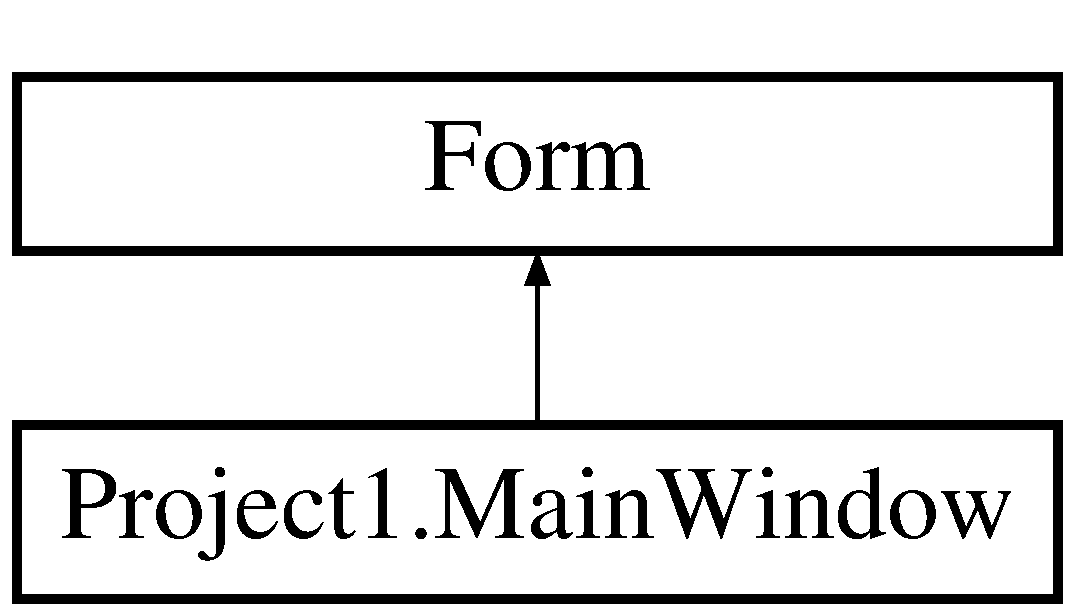
\includegraphics[height=2.000000cm]{classProject1_1_1MainWindow}
\end{center}
\end{figure}
\subsection*{Public Member Functions}
\begin{DoxyCompactItemize}
\item 
\hyperlink{classProject1_1_1MainWindow_ac8ada21cf001233b859c3c8fd34dbd14}{Main\+Window} ()
\begin{DoxyCompactList}\small\item\em Initializes a new instance of the \hyperlink{classProject1_1_1MainWindow}{Main\+Window} class. \end{DoxyCompactList}\end{DoxyCompactItemize}
\subsection*{Protected Member Functions}
\begin{DoxyCompactItemize}
\item 
override void \hyperlink{classProject1_1_1MainWindow_a6a752bcb31d44385e4f21b1e75861615}{Dispose} (bool disposing)
\begin{DoxyCompactList}\small\item\em Clean up any resources being used. \end{DoxyCompactList}\end{DoxyCompactItemize}
\subsection*{Package Functions}
\begin{DoxyCompactItemize}
\item 
void \hyperlink{classProject1_1_1MainWindow_af3d1ecd028cb95773e1c1eec3a28e7ce}{Reload\+Attendees} ()
\begin{DoxyCompactList}\small\item\em Reloads the attendees. \end{DoxyCompactList}\item 
void \hyperlink{classProject1_1_1MainWindow_aef6b435caef02f80d3f3752684cf00f6}{Reload\+Events} ()
\begin{DoxyCompactList}\small\item\em Reloads the events. \end{DoxyCompactList}\end{DoxyCompactItemize}
\subsection*{Static Package Attributes}
\begin{DoxyCompactItemize}
\item 
static List$<$ \hyperlink{classProject1_1_1Event}{Event} $>$ \hyperlink{classProject1_1_1MainWindow_ae3afd09951104ecaa17ed586dd934249}{Events\+List} = new List$<$\hyperlink{classProject1_1_1Event}{Event}$>$()
\begin{DoxyCompactList}\small\item\em The events list \end{DoxyCompactList}\end{DoxyCompactItemize}
\subsection*{Private Member Functions}
\begin{DoxyCompactItemize}
\item 
void \hyperlink{classProject1_1_1MainWindow_acddeca5d53ed4be2a81351d1681b4cb5}{add\+Event\+Button\+\_\+\+Click} (object sender, Event\+Args e)
\begin{DoxyCompactList}\small\item\em Ask for event infromation in a new window and updates listbox for available events. \end{DoxyCompactList}\item 
void \hyperlink{classProject1_1_1MainWindow_a70b3092e895f756ceda7a95309581fe5}{availability\+Button\+\_\+\+Click} (object sender, Event\+Args e)
\begin{DoxyCompactList}\small\item\em If no list\+Box item is selected, prompt the user for a listbox selection. From that listbox selection, prompt the user for available dates for the selected event in a new window. \end{DoxyCompactList}\item 
void \hyperlink{classProject1_1_1MainWindow_a31c174049fa92aa29587cf81f7749bd3}{Main\+Window\+\_\+\+Load} (object sender, Event\+Args e)
\begin{DoxyCompactList}\small\item\em Handles the Load event of the \hyperlink{classProject1_1_1MainWindow}{Main\+Window} control. \end{DoxyCompactList}\item 
void \hyperlink{classProject1_1_1MainWindow_a9204f8ca23668b22fa23b4fa44b3ae67}{check\+Box1\+\_\+\+Checked\+Changed} (object sender, Event\+Args e)
\begin{DoxyCompactList}\small\item\em Handles the Checked\+Changed event of the check\+Box1 control. \end{DoxyCompactList}\item 
void \hyperlink{classProject1_1_1MainWindow_a3062c1009a2a7a443176cf874520eebe}{Initialize\+Component} ()
\begin{DoxyCompactList}\small\item\em Required method for Designer support -\/ do not modify the contents of this method with the code editor. \end{DoxyCompactList}\end{DoxyCompactItemize}
\subsection*{Private Attributes}
\begin{DoxyCompactItemize}
\item 
System.\+Component\+Model.\+I\+Container \hyperlink{classProject1_1_1MainWindow_ab73af7a7685fb735923099a87cc5c81a}{components} = null
\begin{DoxyCompactList}\small\item\em Required designer variable. \end{DoxyCompactList}\item 
System.\+Windows.\+Forms.\+Button \hyperlink{classProject1_1_1MainWindow_a3d99b09991f5611424ec9886d8805fce}{add\+Event\+Button}
\item 
System.\+Windows.\+Forms.\+Button \hyperlink{classProject1_1_1MainWindow_a3e34c89029ddf939d607ea8638e444c8}{availability\+Button}
\item 
System.\+Windows.\+Forms.\+List\+View \hyperlink{classProject1_1_1MainWindow_a87e159953fb2bc0cb9276dc85f2e7979}{attendee\+View}
\item 
System.\+Windows.\+Forms.\+Column\+Header \hyperlink{classProject1_1_1MainWindow_a2814c0939a2ecfdcb2506f83fcfff080}{column\+Header3}
\item 
System.\+Windows.\+Forms.\+Column\+Header \hyperlink{classProject1_1_1MainWindow_acaaac5d2776ef69f8e9abbb61b06ee64}{column\+Header7}
\item 
System.\+Windows.\+Forms.\+Column\+Header \hyperlink{classProject1_1_1MainWindow_aaed23b23d4df062fe99afdee1730e800}{column\+Header11}
\item 
System.\+Windows.\+Forms.\+Check\+Box \hyperlink{classProject1_1_1MainWindow_a2e6cf3cf871c168672d16d8c12211047}{check\+Box1}
\item 
System.\+Windows.\+Forms.\+List\+View \hyperlink{classProject1_1_1MainWindow_a48288e76cf64892256e3ec2f3173bcb8}{event\+View}
\item 
System.\+Windows.\+Forms.\+Column\+Header \hyperlink{classProject1_1_1MainWindow_a8cc8ae19b57ec667fa7cc09ed7446056}{column\+Header5}
\item 
System.\+Windows.\+Forms.\+Column\+Header \hyperlink{classProject1_1_1MainWindow_a5041ff81bbef58fc72cb0914afa984ea}{column\+Header6}
\item 
System.\+Windows.\+Forms.\+Column\+Header \hyperlink{classProject1_1_1MainWindow_ac624f584eb3fbe129389e2b3e287f596}{column\+Header10}
\item 
System.\+Windows.\+Forms.\+Column\+Header \hyperlink{classProject1_1_1MainWindow_a7ad81e39a25ae4972c28b1d805b827a9}{column\+Header12}
\item 
System.\+Windows.\+Forms.\+Column\+Header \hyperlink{classProject1_1_1MainWindow_ab661e6cae54e37f16fed3117b6b038e6}{column\+Header13}
\end{DoxyCompactItemize}


\subsection{Detailed Description}
The Main Window form 

\begin{DoxySeeAlso}{See also}
System.\+Windows.\+Forms.\+Form


\end{DoxySeeAlso}


\subsection{Constructor \& Destructor Documentation}
\mbox{\Hypertarget{classProject1_1_1MainWindow_ac8ada21cf001233b859c3c8fd34dbd14}\label{classProject1_1_1MainWindow_ac8ada21cf001233b859c3c8fd34dbd14}} 
\index{Project1\+::\+Main\+Window@{Project1\+::\+Main\+Window}!Main\+Window@{Main\+Window}}
\index{Main\+Window@{Main\+Window}!Project1\+::\+Main\+Window@{Project1\+::\+Main\+Window}}
\subsubsection{\texorpdfstring{Main\+Window()}{MainWindow()}}
{\footnotesize\ttfamily Project1.\+Main\+Window.\+Main\+Window (\begin{DoxyParamCaption}{ }\end{DoxyParamCaption})\hspace{0.3cm}{\ttfamily [inline]}}



Initializes a new instance of the \hyperlink{classProject1_1_1MainWindow}{Main\+Window} class. 



\subsection{Member Function Documentation}
\mbox{\Hypertarget{classProject1_1_1MainWindow_acddeca5d53ed4be2a81351d1681b4cb5}\label{classProject1_1_1MainWindow_acddeca5d53ed4be2a81351d1681b4cb5}} 
\index{Project1\+::\+Main\+Window@{Project1\+::\+Main\+Window}!add\+Event\+Button\+\_\+\+Click@{add\+Event\+Button\+\_\+\+Click}}
\index{add\+Event\+Button\+\_\+\+Click@{add\+Event\+Button\+\_\+\+Click}!Project1\+::\+Main\+Window@{Project1\+::\+Main\+Window}}
\subsubsection{\texorpdfstring{add\+Event\+Button\+\_\+\+Click()}{addEventButton\_Click()}}
{\footnotesize\ttfamily void Project1.\+Main\+Window.\+add\+Event\+Button\+\_\+\+Click (\begin{DoxyParamCaption}\item[{object}]{sender,  }\item[{Event\+Args}]{e }\end{DoxyParamCaption})\hspace{0.3cm}{\ttfamily [inline]}, {\ttfamily [private]}}



Ask for event infromation in a new window and updates listbox for available events. 


\begin{DoxyParams}{Parameters}
{\em sender} & The source of the event.\\
\hline
{\em e} & The Event\+Args instance containing the event data.\\
\hline
\end{DoxyParams}
\mbox{\Hypertarget{classProject1_1_1MainWindow_a70b3092e895f756ceda7a95309581fe5}\label{classProject1_1_1MainWindow_a70b3092e895f756ceda7a95309581fe5}} 
\index{Project1\+::\+Main\+Window@{Project1\+::\+Main\+Window}!availability\+Button\+\_\+\+Click@{availability\+Button\+\_\+\+Click}}
\index{availability\+Button\+\_\+\+Click@{availability\+Button\+\_\+\+Click}!Project1\+::\+Main\+Window@{Project1\+::\+Main\+Window}}
\subsubsection{\texorpdfstring{availability\+Button\+\_\+\+Click()}{availabilityButton\_Click()}}
{\footnotesize\ttfamily void Project1.\+Main\+Window.\+availability\+Button\+\_\+\+Click (\begin{DoxyParamCaption}\item[{object}]{sender,  }\item[{Event\+Args}]{e }\end{DoxyParamCaption})\hspace{0.3cm}{\ttfamily [inline]}, {\ttfamily [private]}}



If no list\+Box item is selected, prompt the user for a listbox selection. From that listbox selection, prompt the user for available dates for the selected event in a new window. 


\begin{DoxyParams}{Parameters}
{\em sender} & The source of the event.\\
\hline
{\em e} & The Event\+Args instance containing the event data.\\
\hline
\end{DoxyParams}
\mbox{\Hypertarget{classProject1_1_1MainWindow_a9204f8ca23668b22fa23b4fa44b3ae67}\label{classProject1_1_1MainWindow_a9204f8ca23668b22fa23b4fa44b3ae67}} 
\index{Project1\+::\+Main\+Window@{Project1\+::\+Main\+Window}!check\+Box1\+\_\+\+Checked\+Changed@{check\+Box1\+\_\+\+Checked\+Changed}}
\index{check\+Box1\+\_\+\+Checked\+Changed@{check\+Box1\+\_\+\+Checked\+Changed}!Project1\+::\+Main\+Window@{Project1\+::\+Main\+Window}}
\subsubsection{\texorpdfstring{check\+Box1\+\_\+\+Checked\+Changed()}{checkBox1\_CheckedChanged()}}
{\footnotesize\ttfamily void Project1.\+Main\+Window.\+check\+Box1\+\_\+\+Checked\+Changed (\begin{DoxyParamCaption}\item[{object}]{sender,  }\item[{Event\+Args}]{e }\end{DoxyParamCaption})\hspace{0.3cm}{\ttfamily [inline]}, {\ttfamily [private]}}



Handles the Checked\+Changed event of the check\+Box1 control. 


\begin{DoxyParams}{Parameters}
{\em sender} & The source of the event.\\
\hline
{\em e} & The Event\+Args instance containing the event data.\\
\hline
\end{DoxyParams}
\mbox{\Hypertarget{classProject1_1_1MainWindow_a6a752bcb31d44385e4f21b1e75861615}\label{classProject1_1_1MainWindow_a6a752bcb31d44385e4f21b1e75861615}} 
\index{Project1\+::\+Main\+Window@{Project1\+::\+Main\+Window}!Dispose@{Dispose}}
\index{Dispose@{Dispose}!Project1\+::\+Main\+Window@{Project1\+::\+Main\+Window}}
\subsubsection{\texorpdfstring{Dispose()}{Dispose()}}
{\footnotesize\ttfamily override void Project1.\+Main\+Window.\+Dispose (\begin{DoxyParamCaption}\item[{bool}]{disposing }\end{DoxyParamCaption})\hspace{0.3cm}{\ttfamily [inline]}, {\ttfamily [protected]}}



Clean up any resources being used. 


\begin{DoxyParams}{Parameters}
{\em disposing} & true if managed resources should be disposed; otherwise, false.\\
\hline
\end{DoxyParams}
\mbox{\Hypertarget{classProject1_1_1MainWindow_a3062c1009a2a7a443176cf874520eebe}\label{classProject1_1_1MainWindow_a3062c1009a2a7a443176cf874520eebe}} 
\index{Project1\+::\+Main\+Window@{Project1\+::\+Main\+Window}!Initialize\+Component@{Initialize\+Component}}
\index{Initialize\+Component@{Initialize\+Component}!Project1\+::\+Main\+Window@{Project1\+::\+Main\+Window}}
\subsubsection{\texorpdfstring{Initialize\+Component()}{InitializeComponent()}}
{\footnotesize\ttfamily void Project1.\+Main\+Window.\+Initialize\+Component (\begin{DoxyParamCaption}{ }\end{DoxyParamCaption})\hspace{0.3cm}{\ttfamily [inline]}, {\ttfamily [private]}}



Required method for Designer support -\/ do not modify the contents of this method with the code editor. 

\mbox{\Hypertarget{classProject1_1_1MainWindow_a31c174049fa92aa29587cf81f7749bd3}\label{classProject1_1_1MainWindow_a31c174049fa92aa29587cf81f7749bd3}} 
\index{Project1\+::\+Main\+Window@{Project1\+::\+Main\+Window}!Main\+Window\+\_\+\+Load@{Main\+Window\+\_\+\+Load}}
\index{Main\+Window\+\_\+\+Load@{Main\+Window\+\_\+\+Load}!Project1\+::\+Main\+Window@{Project1\+::\+Main\+Window}}
\subsubsection{\texorpdfstring{Main\+Window\+\_\+\+Load()}{MainWindow\_Load()}}
{\footnotesize\ttfamily void Project1.\+Main\+Window.\+Main\+Window\+\_\+\+Load (\begin{DoxyParamCaption}\item[{object}]{sender,  }\item[{Event\+Args}]{e }\end{DoxyParamCaption})\hspace{0.3cm}{\ttfamily [inline]}, {\ttfamily [private]}}



Handles the Load event of the \hyperlink{classProject1_1_1MainWindow}{Main\+Window} control. 


\begin{DoxyParams}{Parameters}
{\em sender} & The source of the event.\\
\hline
{\em e} & The Event\+Args instance containing the event data.\\
\hline
\end{DoxyParams}
\mbox{\Hypertarget{classProject1_1_1MainWindow_af3d1ecd028cb95773e1c1eec3a28e7ce}\label{classProject1_1_1MainWindow_af3d1ecd028cb95773e1c1eec3a28e7ce}} 
\index{Project1\+::\+Main\+Window@{Project1\+::\+Main\+Window}!Reload\+Attendees@{Reload\+Attendees}}
\index{Reload\+Attendees@{Reload\+Attendees}!Project1\+::\+Main\+Window@{Project1\+::\+Main\+Window}}
\subsubsection{\texorpdfstring{Reload\+Attendees()}{ReloadAttendees()}}
{\footnotesize\ttfamily void Project1.\+Main\+Window.\+Reload\+Attendees (\begin{DoxyParamCaption}{ }\end{DoxyParamCaption})\hspace{0.3cm}{\ttfamily [inline]}, {\ttfamily [package]}}



Reloads the attendees. 

\mbox{\Hypertarget{classProject1_1_1MainWindow_aef6b435caef02f80d3f3752684cf00f6}\label{classProject1_1_1MainWindow_aef6b435caef02f80d3f3752684cf00f6}} 
\index{Project1\+::\+Main\+Window@{Project1\+::\+Main\+Window}!Reload\+Events@{Reload\+Events}}
\index{Reload\+Events@{Reload\+Events}!Project1\+::\+Main\+Window@{Project1\+::\+Main\+Window}}
\subsubsection{\texorpdfstring{Reload\+Events()}{ReloadEvents()}}
{\footnotesize\ttfamily void Project1.\+Main\+Window.\+Reload\+Events (\begin{DoxyParamCaption}{ }\end{DoxyParamCaption})\hspace{0.3cm}{\ttfamily [inline]}, {\ttfamily [package]}}



Reloads the events. 



\subsection{Member Data Documentation}
\mbox{\Hypertarget{classProject1_1_1MainWindow_a3d99b09991f5611424ec9886d8805fce}\label{classProject1_1_1MainWindow_a3d99b09991f5611424ec9886d8805fce}} 
\index{Project1\+::\+Main\+Window@{Project1\+::\+Main\+Window}!add\+Event\+Button@{add\+Event\+Button}}
\index{add\+Event\+Button@{add\+Event\+Button}!Project1\+::\+Main\+Window@{Project1\+::\+Main\+Window}}
\subsubsection{\texorpdfstring{add\+Event\+Button}{addEventButton}}
{\footnotesize\ttfamily System.\+Windows.\+Forms.\+Button Project1.\+Main\+Window.\+add\+Event\+Button\hspace{0.3cm}{\ttfamily [private]}}

\mbox{\Hypertarget{classProject1_1_1MainWindow_a87e159953fb2bc0cb9276dc85f2e7979}\label{classProject1_1_1MainWindow_a87e159953fb2bc0cb9276dc85f2e7979}} 
\index{Project1\+::\+Main\+Window@{Project1\+::\+Main\+Window}!attendee\+View@{attendee\+View}}
\index{attendee\+View@{attendee\+View}!Project1\+::\+Main\+Window@{Project1\+::\+Main\+Window}}
\subsubsection{\texorpdfstring{attendee\+View}{attendeeView}}
{\footnotesize\ttfamily System.\+Windows.\+Forms.\+List\+View Project1.\+Main\+Window.\+attendee\+View\hspace{0.3cm}{\ttfamily [private]}}

\mbox{\Hypertarget{classProject1_1_1MainWindow_a3e34c89029ddf939d607ea8638e444c8}\label{classProject1_1_1MainWindow_a3e34c89029ddf939d607ea8638e444c8}} 
\index{Project1\+::\+Main\+Window@{Project1\+::\+Main\+Window}!availability\+Button@{availability\+Button}}
\index{availability\+Button@{availability\+Button}!Project1\+::\+Main\+Window@{Project1\+::\+Main\+Window}}
\subsubsection{\texorpdfstring{availability\+Button}{availabilityButton}}
{\footnotesize\ttfamily System.\+Windows.\+Forms.\+Button Project1.\+Main\+Window.\+availability\+Button\hspace{0.3cm}{\ttfamily [private]}}

\mbox{\Hypertarget{classProject1_1_1MainWindow_a2e6cf3cf871c168672d16d8c12211047}\label{classProject1_1_1MainWindow_a2e6cf3cf871c168672d16d8c12211047}} 
\index{Project1\+::\+Main\+Window@{Project1\+::\+Main\+Window}!check\+Box1@{check\+Box1}}
\index{check\+Box1@{check\+Box1}!Project1\+::\+Main\+Window@{Project1\+::\+Main\+Window}}
\subsubsection{\texorpdfstring{check\+Box1}{checkBox1}}
{\footnotesize\ttfamily System.\+Windows.\+Forms.\+Check\+Box Project1.\+Main\+Window.\+check\+Box1\hspace{0.3cm}{\ttfamily [private]}}

\mbox{\Hypertarget{classProject1_1_1MainWindow_ac624f584eb3fbe129389e2b3e287f596}\label{classProject1_1_1MainWindow_ac624f584eb3fbe129389e2b3e287f596}} 
\index{Project1\+::\+Main\+Window@{Project1\+::\+Main\+Window}!column\+Header10@{column\+Header10}}
\index{column\+Header10@{column\+Header10}!Project1\+::\+Main\+Window@{Project1\+::\+Main\+Window}}
\subsubsection{\texorpdfstring{column\+Header10}{columnHeader10}}
{\footnotesize\ttfamily System.\+Windows.\+Forms.\+Column\+Header Project1.\+Main\+Window.\+column\+Header10\hspace{0.3cm}{\ttfamily [private]}}

\mbox{\Hypertarget{classProject1_1_1MainWindow_aaed23b23d4df062fe99afdee1730e800}\label{classProject1_1_1MainWindow_aaed23b23d4df062fe99afdee1730e800}} 
\index{Project1\+::\+Main\+Window@{Project1\+::\+Main\+Window}!column\+Header11@{column\+Header11}}
\index{column\+Header11@{column\+Header11}!Project1\+::\+Main\+Window@{Project1\+::\+Main\+Window}}
\subsubsection{\texorpdfstring{column\+Header11}{columnHeader11}}
{\footnotesize\ttfamily System.\+Windows.\+Forms.\+Column\+Header Project1.\+Main\+Window.\+column\+Header11\hspace{0.3cm}{\ttfamily [private]}}

\mbox{\Hypertarget{classProject1_1_1MainWindow_a7ad81e39a25ae4972c28b1d805b827a9}\label{classProject1_1_1MainWindow_a7ad81e39a25ae4972c28b1d805b827a9}} 
\index{Project1\+::\+Main\+Window@{Project1\+::\+Main\+Window}!column\+Header12@{column\+Header12}}
\index{column\+Header12@{column\+Header12}!Project1\+::\+Main\+Window@{Project1\+::\+Main\+Window}}
\subsubsection{\texorpdfstring{column\+Header12}{columnHeader12}}
{\footnotesize\ttfamily System.\+Windows.\+Forms.\+Column\+Header Project1.\+Main\+Window.\+column\+Header12\hspace{0.3cm}{\ttfamily [private]}}

\mbox{\Hypertarget{classProject1_1_1MainWindow_ab661e6cae54e37f16fed3117b6b038e6}\label{classProject1_1_1MainWindow_ab661e6cae54e37f16fed3117b6b038e6}} 
\index{Project1\+::\+Main\+Window@{Project1\+::\+Main\+Window}!column\+Header13@{column\+Header13}}
\index{column\+Header13@{column\+Header13}!Project1\+::\+Main\+Window@{Project1\+::\+Main\+Window}}
\subsubsection{\texorpdfstring{column\+Header13}{columnHeader13}}
{\footnotesize\ttfamily System.\+Windows.\+Forms.\+Column\+Header Project1.\+Main\+Window.\+column\+Header13\hspace{0.3cm}{\ttfamily [private]}}

\mbox{\Hypertarget{classProject1_1_1MainWindow_a2814c0939a2ecfdcb2506f83fcfff080}\label{classProject1_1_1MainWindow_a2814c0939a2ecfdcb2506f83fcfff080}} 
\index{Project1\+::\+Main\+Window@{Project1\+::\+Main\+Window}!column\+Header3@{column\+Header3}}
\index{column\+Header3@{column\+Header3}!Project1\+::\+Main\+Window@{Project1\+::\+Main\+Window}}
\subsubsection{\texorpdfstring{column\+Header3}{columnHeader3}}
{\footnotesize\ttfamily System.\+Windows.\+Forms.\+Column\+Header Project1.\+Main\+Window.\+column\+Header3\hspace{0.3cm}{\ttfamily [private]}}

\mbox{\Hypertarget{classProject1_1_1MainWindow_a8cc8ae19b57ec667fa7cc09ed7446056}\label{classProject1_1_1MainWindow_a8cc8ae19b57ec667fa7cc09ed7446056}} 
\index{Project1\+::\+Main\+Window@{Project1\+::\+Main\+Window}!column\+Header5@{column\+Header5}}
\index{column\+Header5@{column\+Header5}!Project1\+::\+Main\+Window@{Project1\+::\+Main\+Window}}
\subsubsection{\texorpdfstring{column\+Header5}{columnHeader5}}
{\footnotesize\ttfamily System.\+Windows.\+Forms.\+Column\+Header Project1.\+Main\+Window.\+column\+Header5\hspace{0.3cm}{\ttfamily [private]}}

\mbox{\Hypertarget{classProject1_1_1MainWindow_a5041ff81bbef58fc72cb0914afa984ea}\label{classProject1_1_1MainWindow_a5041ff81bbef58fc72cb0914afa984ea}} 
\index{Project1\+::\+Main\+Window@{Project1\+::\+Main\+Window}!column\+Header6@{column\+Header6}}
\index{column\+Header6@{column\+Header6}!Project1\+::\+Main\+Window@{Project1\+::\+Main\+Window}}
\subsubsection{\texorpdfstring{column\+Header6}{columnHeader6}}
{\footnotesize\ttfamily System.\+Windows.\+Forms.\+Column\+Header Project1.\+Main\+Window.\+column\+Header6\hspace{0.3cm}{\ttfamily [private]}}

\mbox{\Hypertarget{classProject1_1_1MainWindow_acaaac5d2776ef69f8e9abbb61b06ee64}\label{classProject1_1_1MainWindow_acaaac5d2776ef69f8e9abbb61b06ee64}} 
\index{Project1\+::\+Main\+Window@{Project1\+::\+Main\+Window}!column\+Header7@{column\+Header7}}
\index{column\+Header7@{column\+Header7}!Project1\+::\+Main\+Window@{Project1\+::\+Main\+Window}}
\subsubsection{\texorpdfstring{column\+Header7}{columnHeader7}}
{\footnotesize\ttfamily System.\+Windows.\+Forms.\+Column\+Header Project1.\+Main\+Window.\+column\+Header7\hspace{0.3cm}{\ttfamily [private]}}

\mbox{\Hypertarget{classProject1_1_1MainWindow_ab73af7a7685fb735923099a87cc5c81a}\label{classProject1_1_1MainWindow_ab73af7a7685fb735923099a87cc5c81a}} 
\index{Project1\+::\+Main\+Window@{Project1\+::\+Main\+Window}!components@{components}}
\index{components@{components}!Project1\+::\+Main\+Window@{Project1\+::\+Main\+Window}}
\subsubsection{\texorpdfstring{components}{components}}
{\footnotesize\ttfamily System.\+Component\+Model.\+I\+Container Project1.\+Main\+Window.\+components = null\hspace{0.3cm}{\ttfamily [private]}}



Required designer variable. 

\mbox{\Hypertarget{classProject1_1_1MainWindow_ae3afd09951104ecaa17ed586dd934249}\label{classProject1_1_1MainWindow_ae3afd09951104ecaa17ed586dd934249}} 
\index{Project1\+::\+Main\+Window@{Project1\+::\+Main\+Window}!Events\+List@{Events\+List}}
\index{Events\+List@{Events\+List}!Project1\+::\+Main\+Window@{Project1\+::\+Main\+Window}}
\subsubsection{\texorpdfstring{Events\+List}{EventsList}}
{\footnotesize\ttfamily List$<$\hyperlink{classProject1_1_1Event}{Event}$>$ Project1.\+Main\+Window.\+Events\+List = new List$<$\hyperlink{classProject1_1_1Event}{Event}$>$()\hspace{0.3cm}{\ttfamily [static]}, {\ttfamily [package]}}



The events list 

\mbox{\Hypertarget{classProject1_1_1MainWindow_a48288e76cf64892256e3ec2f3173bcb8}\label{classProject1_1_1MainWindow_a48288e76cf64892256e3ec2f3173bcb8}} 
\index{Project1\+::\+Main\+Window@{Project1\+::\+Main\+Window}!event\+View@{event\+View}}
\index{event\+View@{event\+View}!Project1\+::\+Main\+Window@{Project1\+::\+Main\+Window}}
\subsubsection{\texorpdfstring{event\+View}{eventView}}
{\footnotesize\ttfamily System.\+Windows.\+Forms.\+List\+View Project1.\+Main\+Window.\+event\+View\hspace{0.3cm}{\ttfamily [private]}}



The documentation for this class was generated from the following files\+:\begin{DoxyCompactItemize}
\item 
Project1/\hyperlink{MainWindow_8cs}{Main\+Window.\+cs}\item 
Project1/\hyperlink{MainWindow_8Designer_8cs}{Main\+Window.\+Designer.\+cs}\end{DoxyCompactItemize}

\hypertarget{classProject1_1_1Program}{}\section{Project1.\+Program Class Reference}
\label{classProject1_1_1Program}\index{Project1.\+Program@{Project1.\+Program}}
\subsection*{Static Private Member Functions}
\begin{DoxyCompactItemize}
\item 
static void \hyperlink{classProject1_1_1Program_a41c8e8ccb50be0b9beb690ea31883d3a}{Main} ()
\begin{DoxyCompactList}\small\item\em The main entry point for the application. \end{DoxyCompactList}\end{DoxyCompactItemize}


\subsection{Member Function Documentation}
\mbox{\Hypertarget{classProject1_1_1Program_a41c8e8ccb50be0b9beb690ea31883d3a}\label{classProject1_1_1Program_a41c8e8ccb50be0b9beb690ea31883d3a}} 
\index{Project1\+::\+Program@{Project1\+::\+Program}!Main@{Main}}
\index{Main@{Main}!Project1\+::\+Program@{Project1\+::\+Program}}
\subsubsection{\texorpdfstring{Main()}{Main()}}
{\footnotesize\ttfamily static void Project1.\+Program.\+Main (\begin{DoxyParamCaption}{ }\end{DoxyParamCaption})\hspace{0.3cm}{\ttfamily [inline]}, {\ttfamily [static]}, {\ttfamily [private]}}



The main entry point for the application. 



The documentation for this class was generated from the following file\+:\begin{DoxyCompactItemize}
\item 
Project1/\hyperlink{Program_8cs}{Program.\+cs}\end{DoxyCompactItemize}

\hypertarget{classProject1_1_1Storage}{}\section{Project1.\+Storage Class Reference}
\label{classProject1_1_1Storage}\index{Project1.\+Storage@{Project1.\+Storage}}


Class for helping with file storage/reading  


\subsection*{Static Package Functions}
\begin{DoxyCompactItemize}
\item 
static String \hyperlink{classProject1_1_1Storage_a609f09f2cea1638321ac856303b7837d}{Times\+Formatted} (Date\+Time\mbox{[}$\,$\mbox{]} times, bool mode24=false)
\begin{DoxyCompactList}\small\item\em Formats a Date\+Time array into a string \end{DoxyCompactList}\item 
static void \hyperlink{classProject1_1_1Storage_ae01896659ba07c9e623c37d3ed1caaef}{Add\+Event} (\hyperlink{classProject1_1_1Event}{Event} ev)
\begin{DoxyCompactList}\small\item\em Adds \hyperlink{classProject1_1_1Event}{Event} to file. Output Format\+: user\+\_\+name event\+\_\+name event\+\_\+time \mbox{[}times available\mbox{]} separated by a , \end{DoxyCompactList}\item 
static void \hyperlink{classProject1_1_1Storage_a565feda8803f2fccc4e5a3335903e4fc}{Add\+Attendee} (\hyperlink{classProject1_1_1Attendee}{Attendee} attendee)
\begin{DoxyCompactList}\small\item\em Adds the attendee to file. Format\+: attendee\+Name event\+Name \mbox{[}times\mbox{]} \end{DoxyCompactList}\item 
static \hyperlink{classProject1_1_1Attendee}{Attendee} \hyperlink{classProject1_1_1Storage_a4aebfb33e4df6b8694853cd7c68c4d56}{Read\+Attendee} (string\mbox{[}$\,$\mbox{]} items)
\begin{DoxyCompactList}\small\item\em Reads attendee from a string array \end{DoxyCompactList}\item 
static \hyperlink{classProject1_1_1Event}{Event} \hyperlink{classProject1_1_1Storage_adba708b66c28fbd3e6dff0fb2117d050}{Read\+Event} (string\mbox{[}$\,$\mbox{]} items)
\begin{DoxyCompactList}\small\item\em Reads the event from a string array \end{DoxyCompactList}\end{DoxyCompactItemize}
\subsection*{Static Private Member Functions}
\begin{DoxyCompactItemize}
\item 
static Date\+Time \mbox{[}$\,$\mbox{]} \hyperlink{classProject1_1_1Storage_a376dc3238d3e8ab23781d5401e428865}{Read\+Times} (string\mbox{[}$\,$\mbox{]} times)
\begin{DoxyCompactList}\small\item\em Reads the times. \end{DoxyCompactList}\end{DoxyCompactItemize}


\subsection{Detailed Description}
Class for helping with file storage/reading 



\subsection{Member Function Documentation}
\mbox{\Hypertarget{classProject1_1_1Storage_a565feda8803f2fccc4e5a3335903e4fc}\label{classProject1_1_1Storage_a565feda8803f2fccc4e5a3335903e4fc}} 
\index{Project1\+::\+Storage@{Project1\+::\+Storage}!Add\+Attendee@{Add\+Attendee}}
\index{Add\+Attendee@{Add\+Attendee}!Project1\+::\+Storage@{Project1\+::\+Storage}}
\subsubsection{\texorpdfstring{Add\+Attendee()}{AddAttendee()}}
{\footnotesize\ttfamily static void Project1.\+Storage.\+Add\+Attendee (\begin{DoxyParamCaption}\item[{\hyperlink{classProject1_1_1Attendee}{Attendee}}]{attendee }\end{DoxyParamCaption})\hspace{0.3cm}{\ttfamily [inline]}, {\ttfamily [static]}, {\ttfamily [package]}}



Adds the attendee to file. Format\+: attendee\+Name event\+Name \mbox{[}times\mbox{]} 


\begin{DoxyParams}{Parameters}
{\em attendee} & The attendee.\\
\hline
\end{DoxyParams}
\mbox{\Hypertarget{classProject1_1_1Storage_ae01896659ba07c9e623c37d3ed1caaef}\label{classProject1_1_1Storage_ae01896659ba07c9e623c37d3ed1caaef}} 
\index{Project1\+::\+Storage@{Project1\+::\+Storage}!Add\+Event@{Add\+Event}}
\index{Add\+Event@{Add\+Event}!Project1\+::\+Storage@{Project1\+::\+Storage}}
\subsubsection{\texorpdfstring{Add\+Event()}{AddEvent()}}
{\footnotesize\ttfamily static void Project1.\+Storage.\+Add\+Event (\begin{DoxyParamCaption}\item[{\hyperlink{classProject1_1_1Event}{Event}}]{ev }\end{DoxyParamCaption})\hspace{0.3cm}{\ttfamily [inline]}, {\ttfamily [static]}, {\ttfamily [package]}}



Adds \hyperlink{classProject1_1_1Event}{Event} to file. Output Format\+: user\+\_\+name event\+\_\+name event\+\_\+time \mbox{[}times available\mbox{]} separated by a , 


\begin{DoxyParams}{Parameters}
{\em ev} & The ev.\\
\hline
\end{DoxyParams}
\mbox{\Hypertarget{classProject1_1_1Storage_a4aebfb33e4df6b8694853cd7c68c4d56}\label{classProject1_1_1Storage_a4aebfb33e4df6b8694853cd7c68c4d56}} 
\index{Project1\+::\+Storage@{Project1\+::\+Storage}!Read\+Attendee@{Read\+Attendee}}
\index{Read\+Attendee@{Read\+Attendee}!Project1\+::\+Storage@{Project1\+::\+Storage}}
\subsubsection{\texorpdfstring{Read\+Attendee()}{ReadAttendee()}}
{\footnotesize\ttfamily static \hyperlink{classProject1_1_1Attendee}{Attendee} Project1.\+Storage.\+Read\+Attendee (\begin{DoxyParamCaption}\item[{string \mbox{[}$\,$\mbox{]}}]{items }\end{DoxyParamCaption})\hspace{0.3cm}{\ttfamily [inline]}, {\ttfamily [static]}, {\ttfamily [package]}}



Reads attendee from a string array 


\begin{DoxyParams}{Parameters}
{\em items} & The items.\\
\hline
\end{DoxyParams}
\begin{DoxyReturn}{Returns}

\end{DoxyReturn}
\mbox{\Hypertarget{classProject1_1_1Storage_adba708b66c28fbd3e6dff0fb2117d050}\label{classProject1_1_1Storage_adba708b66c28fbd3e6dff0fb2117d050}} 
\index{Project1\+::\+Storage@{Project1\+::\+Storage}!Read\+Event@{Read\+Event}}
\index{Read\+Event@{Read\+Event}!Project1\+::\+Storage@{Project1\+::\+Storage}}
\subsubsection{\texorpdfstring{Read\+Event()}{ReadEvent()}}
{\footnotesize\ttfamily static \hyperlink{classProject1_1_1Event}{Event} Project1.\+Storage.\+Read\+Event (\begin{DoxyParamCaption}\item[{string \mbox{[}$\,$\mbox{]}}]{items }\end{DoxyParamCaption})\hspace{0.3cm}{\ttfamily [inline]}, {\ttfamily [static]}, {\ttfamily [package]}}



Reads the event from a string array 


\begin{DoxyParams}{Parameters}
{\em items} & The items.\\
\hline
\end{DoxyParams}
\begin{DoxyReturn}{Returns}

\end{DoxyReturn}
\mbox{\Hypertarget{classProject1_1_1Storage_a376dc3238d3e8ab23781d5401e428865}\label{classProject1_1_1Storage_a376dc3238d3e8ab23781d5401e428865}} 
\index{Project1\+::\+Storage@{Project1\+::\+Storage}!Read\+Times@{Read\+Times}}
\index{Read\+Times@{Read\+Times}!Project1\+::\+Storage@{Project1\+::\+Storage}}
\subsubsection{\texorpdfstring{Read\+Times()}{ReadTimes()}}
{\footnotesize\ttfamily static Date\+Time \mbox{[}$\,$\mbox{]} Project1.\+Storage.\+Read\+Times (\begin{DoxyParamCaption}\item[{string \mbox{[}$\,$\mbox{]}}]{times }\end{DoxyParamCaption})\hspace{0.3cm}{\ttfamily [inline]}, {\ttfamily [static]}, {\ttfamily [private]}}



Reads the times. 


\begin{DoxyParams}{Parameters}
{\em times} & The times.\\
\hline
\end{DoxyParams}
\begin{DoxyReturn}{Returns}

\end{DoxyReturn}
\mbox{\Hypertarget{classProject1_1_1Storage_a609f09f2cea1638321ac856303b7837d}\label{classProject1_1_1Storage_a609f09f2cea1638321ac856303b7837d}} 
\index{Project1\+::\+Storage@{Project1\+::\+Storage}!Times\+Formatted@{Times\+Formatted}}
\index{Times\+Formatted@{Times\+Formatted}!Project1\+::\+Storage@{Project1\+::\+Storage}}
\subsubsection{\texorpdfstring{Times\+Formatted()}{TimesFormatted()}}
{\footnotesize\ttfamily static String Project1.\+Storage.\+Times\+Formatted (\begin{DoxyParamCaption}\item[{Date\+Time \mbox{[}$\,$\mbox{]}}]{times,  }\item[{bool}]{mode24 = {\ttfamily false} }\end{DoxyParamCaption})\hspace{0.3cm}{\ttfamily [inline]}, {\ttfamily [static]}, {\ttfamily [package]}}



Formats a Date\+Time array into a string 


\begin{DoxyParams}{Parameters}
{\em times} & The times.\\
\hline
{\em mode24} & if set to {\ttfamily true} \mbox{[}mode24\mbox{]}.\\
\hline
\end{DoxyParams}
\begin{DoxyReturn}{Returns}

\end{DoxyReturn}


The documentation for this class was generated from the following file\+:\begin{DoxyCompactItemize}
\item 
Project1/\hyperlink{Storage_8cs}{Storage.\+cs}\end{DoxyCompactItemize}

\chapter{File Documentation}
\hypertarget{Attendee_8cs}{}\section{Project1/\+Attendee.cs File Reference}
\label{Attendee_8cs}\index{Project1/\+Attendee.\+cs@{Project1/\+Attendee.\+cs}}
\subsection*{Classes}
\begin{DoxyCompactItemize}
\item 
class \hyperlink{classProject1_1_1Attendee}{Project1.\+Attendee}
\begin{DoxyCompactList}\small\item\em \hyperlink{classProject1_1_1Attendee}{Attendee} class \end{DoxyCompactList}\end{DoxyCompactItemize}
\subsection*{Namespaces}
\begin{DoxyCompactItemize}
\item 
namespace \hyperlink{namespaceProject1}{Project1}
\end{DoxyCompactItemize}

\hypertarget{AvailabilityForm_8cs}{}\section{Project1/\+Availability\+Form.cs File Reference}
\label{AvailabilityForm_8cs}\index{Project1/\+Availability\+Form.\+cs@{Project1/\+Availability\+Form.\+cs}}
\subsection*{Classes}
\begin{DoxyCompactItemize}
\item 
class \hyperlink{classProject1_1_1AvailabilityForm}{Project1.\+Availability\+Form}
\begin{DoxyCompactList}\small\item\em Form for adding availability \end{DoxyCompactList}\end{DoxyCompactItemize}
\subsection*{Namespaces}
\begin{DoxyCompactItemize}
\item 
namespace \hyperlink{namespaceProject1}{Project1}
\end{DoxyCompactItemize}

\hypertarget{AvailabilityForm_8Designer_8cs}{}\section{Project1/\+Availability\+Form.Designer.\+cs File Reference}
\label{AvailabilityForm_8Designer_8cs}\index{Project1/\+Availability\+Form.\+Designer.\+cs@{Project1/\+Availability\+Form.\+Designer.\+cs}}
\subsection*{Classes}
\begin{DoxyCompactItemize}
\item 
class \hyperlink{classProject1_1_1AvailabilityForm}{Project1.\+Availability\+Form}
\begin{DoxyCompactList}\small\item\em Form for adding availability \end{DoxyCompactList}\end{DoxyCompactItemize}
\subsection*{Namespaces}
\begin{DoxyCompactItemize}
\item 
namespace \hyperlink{namespaceProject1}{Project1}
\end{DoxyCompactItemize}

\hypertarget{Event_8cs}{}\section{Project1/\+Event.cs File Reference}
\label{Event_8cs}\index{Project1/\+Event.\+cs@{Project1/\+Event.\+cs}}
\subsection*{Classes}
\begin{DoxyCompactItemize}
\item 
class \hyperlink{classProject1_1_1Event}{Project1.\+Event}
\begin{DoxyCompactList}\small\item\em \hyperlink{classProject1_1_1Event}{Event} class \end{DoxyCompactList}\end{DoxyCompactItemize}
\subsection*{Namespaces}
\begin{DoxyCompactItemize}
\item 
namespace \hyperlink{namespaceProject1}{Project1}
\end{DoxyCompactItemize}

\hypertarget{EventInfo_8cs}{}\section{Project1/\+Event\+Info.cs File Reference}
\label{EventInfo_8cs}\index{Project1/\+Event\+Info.\+cs@{Project1/\+Event\+Info.\+cs}}
\subsection*{Classes}
\begin{DoxyCompactItemize}
\item 
class \hyperlink{classProject1_1_1EventInfo}{Project1.\+Event\+Info}
\begin{DoxyCompactList}\small\item\em The event creation form \end{DoxyCompactList}\end{DoxyCompactItemize}
\subsection*{Namespaces}
\begin{DoxyCompactItemize}
\item 
namespace \hyperlink{namespaceProject1}{Project1}
\end{DoxyCompactItemize}

\hypertarget{EventInfo_8Designer_8cs}{}\section{Project1/\+Event\+Info.Designer.\+cs File Reference}
\label{EventInfo_8Designer_8cs}\index{Project1/\+Event\+Info.\+Designer.\+cs@{Project1/\+Event\+Info.\+Designer.\+cs}}
\subsection*{Classes}
\begin{DoxyCompactItemize}
\item 
class \hyperlink{classProject1_1_1EventInfo}{Project1.\+Event\+Info}
\begin{DoxyCompactList}\small\item\em The event creation form \end{DoxyCompactList}\end{DoxyCompactItemize}
\subsection*{Namespaces}
\begin{DoxyCompactItemize}
\item 
namespace \hyperlink{namespaceProject1}{Project1}
\end{DoxyCompactItemize}

\hypertarget{MainWindow_8cs}{}\section{Project1/\+Main\+Window.cs File Reference}
\label{MainWindow_8cs}\index{Project1/\+Main\+Window.\+cs@{Project1/\+Main\+Window.\+cs}}
\subsection*{Classes}
\begin{DoxyCompactItemize}
\item 
class \hyperlink{classProject1_1_1MainWindow}{Project1.\+Main\+Window}
\begin{DoxyCompactList}\small\item\em The Main Window form \end{DoxyCompactList}\end{DoxyCompactItemize}
\subsection*{Namespaces}
\begin{DoxyCompactItemize}
\item 
namespace \hyperlink{namespaceProject1}{Project1}
\end{DoxyCompactItemize}

\hypertarget{MainWindow_8Designer_8cs}{}\section{Project1/\+Main\+Window.Designer.\+cs File Reference}
\label{MainWindow_8Designer_8cs}\index{Project1/\+Main\+Window.\+Designer.\+cs@{Project1/\+Main\+Window.\+Designer.\+cs}}
\subsection*{Classes}
\begin{DoxyCompactItemize}
\item 
class \hyperlink{classProject1_1_1MainWindow}{Project1.\+Main\+Window}
\begin{DoxyCompactList}\small\item\em The Main Window form \end{DoxyCompactList}\end{DoxyCompactItemize}
\subsection*{Namespaces}
\begin{DoxyCompactItemize}
\item 
namespace \hyperlink{namespaceProject1}{Project1}
\end{DoxyCompactItemize}

\hypertarget{Program_8cs}{}\section{Project1/\+Program.cs File Reference}
\label{Program_8cs}\index{Project1/\+Program.\+cs@{Project1/\+Program.\+cs}}
\subsection*{Classes}
\begin{DoxyCompactItemize}
\item 
class \hyperlink{classProject1_1_1Program}{Project1.\+Program}
\end{DoxyCompactItemize}
\subsection*{Namespaces}
\begin{DoxyCompactItemize}
\item 
namespace \hyperlink{namespaceProject1}{Project1}
\end{DoxyCompactItemize}

\hypertarget{Storage_8cs}{}\section{Project1/\+Storage.cs File Reference}
\label{Storage_8cs}\index{Project1/\+Storage.\+cs@{Project1/\+Storage.\+cs}}
\subsection*{Classes}
\begin{DoxyCompactItemize}
\item 
class \hyperlink{classProject1_1_1Storage}{Project1.\+Storage}
\begin{DoxyCompactList}\small\item\em Class for helping with file storage/reading \end{DoxyCompactList}\end{DoxyCompactItemize}
\subsection*{Namespaces}
\begin{DoxyCompactItemize}
\item 
namespace \hyperlink{namespaceProject1}{Project1}
\end{DoxyCompactItemize}

%--- End generated contents ---

% Index
\backmatter
\newpage
\phantomsection
\clearemptydoublepage
\addcontentsline{toc}{chapter}{Index}
\printindex

\end{document}
